
% Default to the notebook output style

    


% Inherit from the specified cell style.




    
\documentclass[11pt]{article}

    
    
    \usepackage[T1]{fontenc}
    % Nicer default font (+ math font) than Computer Modern for most use cases
    \usepackage{mathpazo}

    % Basic figure setup, for now with no caption control since it's done
    % automatically by Pandoc (which extracts ![](path) syntax from Markdown).
    \usepackage{graphicx}
    % We will generate all images so they have a width \maxwidth. This means
    % that they will get their normal width if they fit onto the page, but
    % are scaled down if they would overflow the margins.
    \makeatletter
    \def\maxwidth{\ifdim\Gin@nat@width>\linewidth\linewidth
    \else\Gin@nat@width\fi}
    \makeatother
    \let\Oldincludegraphics\includegraphics
    % Set max figure width to be 80% of text width, for now hardcoded.
    \renewcommand{\includegraphics}[1]{\Oldincludegraphics[width=.8\maxwidth]{#1}}
    % Ensure that by default, figures have no caption (until we provide a
    % proper Figure object with a Caption API and a way to capture that
    % in the conversion process - todo).
    \usepackage{caption}
    \DeclareCaptionLabelFormat{nolabel}{}
    \captionsetup{labelformat=nolabel}

    \usepackage{adjustbox} % Used to constrain images to a maximum size 
    \usepackage{xcolor} % Allow colors to be defined
    \usepackage{enumerate} % Needed for markdown enumerations to work
    \usepackage{geometry} % Used to adjust the document margins
    \usepackage{amsmath} % Equations
    \usepackage{amssymb} % Equations
    \usepackage{textcomp} % defines textquotesingle
    % Hack from http://tex.stackexchange.com/a/47451/13684:
    \AtBeginDocument{%
        \def\PYZsq{\textquotesingle}% Upright quotes in Pygmentized code
    }
    \usepackage{upquote} % Upright quotes for verbatim code
    \usepackage{eurosym} % defines \euro
    \usepackage[mathletters]{ucs} % Extended unicode (utf-8) support
    \usepackage[utf8x]{inputenc} % Allow utf-8 characters in the tex document
    \usepackage{fancyvrb} % verbatim replacement that allows latex
    \usepackage{grffile} % extends the file name processing of package graphics 
                         % to support a larger range 
    % The hyperref package gives us a pdf with properly built
    % internal navigation ('pdf bookmarks' for the table of contents,
    % internal cross-reference links, web links for URLs, etc.)
    \usepackage{hyperref}
    \usepackage{longtable} % longtable support required by pandoc >1.10
    \usepackage{booktabs}  % table support for pandoc > 1.12.2
    \usepackage[inline]{enumitem} % IRkernel/repr support (it uses the enumerate* environment)
    \usepackage[normalem]{ulem} % ulem is needed to support strikethroughs (\sout)
                                % normalem makes italics be italics, not underlines
    

    
    
    % Colors for the hyperref package
    \definecolor{urlcolor}{rgb}{0,.145,.698}
    \definecolor{linkcolor}{rgb}{.71,0.21,0.01}
    \definecolor{citecolor}{rgb}{.12,.54,.11}

    % ANSI colors
    \definecolor{ansi-black}{HTML}{3E424D}
    \definecolor{ansi-black-intense}{HTML}{282C36}
    \definecolor{ansi-red}{HTML}{E75C58}
    \definecolor{ansi-red-intense}{HTML}{B22B31}
    \definecolor{ansi-green}{HTML}{00A250}
    \definecolor{ansi-green-intense}{HTML}{007427}
    \definecolor{ansi-yellow}{HTML}{DDB62B}
    \definecolor{ansi-yellow-intense}{HTML}{B27D12}
    \definecolor{ansi-blue}{HTML}{208FFB}
    \definecolor{ansi-blue-intense}{HTML}{0065CA}
    \definecolor{ansi-magenta}{HTML}{D160C4}
    \definecolor{ansi-magenta-intense}{HTML}{A03196}
    \definecolor{ansi-cyan}{HTML}{60C6C8}
    \definecolor{ansi-cyan-intense}{HTML}{258F8F}
    \definecolor{ansi-white}{HTML}{C5C1B4}
    \definecolor{ansi-white-intense}{HTML}{A1A6B2}

    % commands and environments needed by pandoc snippets
    % extracted from the output of `pandoc -s`
    \providecommand{\tightlist}{%
      \setlength{\itemsep}{0pt}\setlength{\parskip}{0pt}}
    \DefineVerbatimEnvironment{Highlighting}{Verbatim}{commandchars=\\\{\}}
    % Add ',fontsize=\small' for more characters per line
    \newenvironment{Shaded}{}{}
    \newcommand{\KeywordTok}[1]{\textcolor[rgb]{0.00,0.44,0.13}{\textbf{{#1}}}}
    \newcommand{\DataTypeTok}[1]{\textcolor[rgb]{0.56,0.13,0.00}{{#1}}}
    \newcommand{\DecValTok}[1]{\textcolor[rgb]{0.25,0.63,0.44}{{#1}}}
    \newcommand{\BaseNTok}[1]{\textcolor[rgb]{0.25,0.63,0.44}{{#1}}}
    \newcommand{\FloatTok}[1]{\textcolor[rgb]{0.25,0.63,0.44}{{#1}}}
    \newcommand{\CharTok}[1]{\textcolor[rgb]{0.25,0.44,0.63}{{#1}}}
    \newcommand{\StringTok}[1]{\textcolor[rgb]{0.25,0.44,0.63}{{#1}}}
    \newcommand{\CommentTok}[1]{\textcolor[rgb]{0.38,0.63,0.69}{\textit{{#1}}}}
    \newcommand{\OtherTok}[1]{\textcolor[rgb]{0.00,0.44,0.13}{{#1}}}
    \newcommand{\AlertTok}[1]{\textcolor[rgb]{1.00,0.00,0.00}{\textbf{{#1}}}}
    \newcommand{\FunctionTok}[1]{\textcolor[rgb]{0.02,0.16,0.49}{{#1}}}
    \newcommand{\RegionMarkerTok}[1]{{#1}}
    \newcommand{\ErrorTok}[1]{\textcolor[rgb]{1.00,0.00,0.00}{\textbf{{#1}}}}
    \newcommand{\NormalTok}[1]{{#1}}
    
    % Additional commands for more recent versions of Pandoc
    \newcommand{\ConstantTok}[1]{\textcolor[rgb]{0.53,0.00,0.00}{{#1}}}
    \newcommand{\SpecialCharTok}[1]{\textcolor[rgb]{0.25,0.44,0.63}{{#1}}}
    \newcommand{\VerbatimStringTok}[1]{\textcolor[rgb]{0.25,0.44,0.63}{{#1}}}
    \newcommand{\SpecialStringTok}[1]{\textcolor[rgb]{0.73,0.40,0.53}{{#1}}}
    \newcommand{\ImportTok}[1]{{#1}}
    \newcommand{\DocumentationTok}[1]{\textcolor[rgb]{0.73,0.13,0.13}{\textit{{#1}}}}
    \newcommand{\AnnotationTok}[1]{\textcolor[rgb]{0.38,0.63,0.69}{\textbf{\textit{{#1}}}}}
    \newcommand{\CommentVarTok}[1]{\textcolor[rgb]{0.38,0.63,0.69}{\textbf{\textit{{#1}}}}}
    \newcommand{\VariableTok}[1]{\textcolor[rgb]{0.10,0.09,0.49}{{#1}}}
    \newcommand{\ControlFlowTok}[1]{\textcolor[rgb]{0.00,0.44,0.13}{\textbf{{#1}}}}
    \newcommand{\OperatorTok}[1]{\textcolor[rgb]{0.40,0.40,0.40}{{#1}}}
    \newcommand{\BuiltInTok}[1]{{#1}}
    \newcommand{\ExtensionTok}[1]{{#1}}
    \newcommand{\PreprocessorTok}[1]{\textcolor[rgb]{0.74,0.48,0.00}{{#1}}}
    \newcommand{\AttributeTok}[1]{\textcolor[rgb]{0.49,0.56,0.16}{{#1}}}
    \newcommand{\InformationTok}[1]{\textcolor[rgb]{0.38,0.63,0.69}{\textbf{\textit{{#1}}}}}
    \newcommand{\WarningTok}[1]{\textcolor[rgb]{0.38,0.63,0.69}{\textbf{\textit{{#1}}}}}
    
    
    % Define a nice break command that doesn't care if a line doesn't already
    % exist.
    \def\br{\hspace*{\fill} \\* }
    % Math Jax compatability definitions
    \def\gt{>}
    \def\lt{<}
    % Document parameters
    \title{DIP-HW4}
    
    
    

    % Pygments definitions
    
\makeatletter
\def\PY@reset{\let\PY@it=\relax \let\PY@bf=\relax%
    \let\PY@ul=\relax \let\PY@tc=\relax%
    \let\PY@bc=\relax \let\PY@ff=\relax}
\def\PY@tok#1{\csname PY@tok@#1\endcsname}
\def\PY@toks#1+{\ifx\relax#1\empty\else%
    \PY@tok{#1}\expandafter\PY@toks\fi}
\def\PY@do#1{\PY@bc{\PY@tc{\PY@ul{%
    \PY@it{\PY@bf{\PY@ff{#1}}}}}}}
\def\PY#1#2{\PY@reset\PY@toks#1+\relax+\PY@do{#2}}

\expandafter\def\csname PY@tok@w\endcsname{\def\PY@tc##1{\textcolor[rgb]{0.73,0.73,0.73}{##1}}}
\expandafter\def\csname PY@tok@c\endcsname{\let\PY@it=\textit\def\PY@tc##1{\textcolor[rgb]{0.25,0.50,0.50}{##1}}}
\expandafter\def\csname PY@tok@cp\endcsname{\def\PY@tc##1{\textcolor[rgb]{0.74,0.48,0.00}{##1}}}
\expandafter\def\csname PY@tok@k\endcsname{\let\PY@bf=\textbf\def\PY@tc##1{\textcolor[rgb]{0.00,0.50,0.00}{##1}}}
\expandafter\def\csname PY@tok@kp\endcsname{\def\PY@tc##1{\textcolor[rgb]{0.00,0.50,0.00}{##1}}}
\expandafter\def\csname PY@tok@kt\endcsname{\def\PY@tc##1{\textcolor[rgb]{0.69,0.00,0.25}{##1}}}
\expandafter\def\csname PY@tok@o\endcsname{\def\PY@tc##1{\textcolor[rgb]{0.40,0.40,0.40}{##1}}}
\expandafter\def\csname PY@tok@ow\endcsname{\let\PY@bf=\textbf\def\PY@tc##1{\textcolor[rgb]{0.67,0.13,1.00}{##1}}}
\expandafter\def\csname PY@tok@nb\endcsname{\def\PY@tc##1{\textcolor[rgb]{0.00,0.50,0.00}{##1}}}
\expandafter\def\csname PY@tok@nf\endcsname{\def\PY@tc##1{\textcolor[rgb]{0.00,0.00,1.00}{##1}}}
\expandafter\def\csname PY@tok@nc\endcsname{\let\PY@bf=\textbf\def\PY@tc##1{\textcolor[rgb]{0.00,0.00,1.00}{##1}}}
\expandafter\def\csname PY@tok@nn\endcsname{\let\PY@bf=\textbf\def\PY@tc##1{\textcolor[rgb]{0.00,0.00,1.00}{##1}}}
\expandafter\def\csname PY@tok@ne\endcsname{\let\PY@bf=\textbf\def\PY@tc##1{\textcolor[rgb]{0.82,0.25,0.23}{##1}}}
\expandafter\def\csname PY@tok@nv\endcsname{\def\PY@tc##1{\textcolor[rgb]{0.10,0.09,0.49}{##1}}}
\expandafter\def\csname PY@tok@no\endcsname{\def\PY@tc##1{\textcolor[rgb]{0.53,0.00,0.00}{##1}}}
\expandafter\def\csname PY@tok@nl\endcsname{\def\PY@tc##1{\textcolor[rgb]{0.63,0.63,0.00}{##1}}}
\expandafter\def\csname PY@tok@ni\endcsname{\let\PY@bf=\textbf\def\PY@tc##1{\textcolor[rgb]{0.60,0.60,0.60}{##1}}}
\expandafter\def\csname PY@tok@na\endcsname{\def\PY@tc##1{\textcolor[rgb]{0.49,0.56,0.16}{##1}}}
\expandafter\def\csname PY@tok@nt\endcsname{\let\PY@bf=\textbf\def\PY@tc##1{\textcolor[rgb]{0.00,0.50,0.00}{##1}}}
\expandafter\def\csname PY@tok@nd\endcsname{\def\PY@tc##1{\textcolor[rgb]{0.67,0.13,1.00}{##1}}}
\expandafter\def\csname PY@tok@s\endcsname{\def\PY@tc##1{\textcolor[rgb]{0.73,0.13,0.13}{##1}}}
\expandafter\def\csname PY@tok@sd\endcsname{\let\PY@it=\textit\def\PY@tc##1{\textcolor[rgb]{0.73,0.13,0.13}{##1}}}
\expandafter\def\csname PY@tok@si\endcsname{\let\PY@bf=\textbf\def\PY@tc##1{\textcolor[rgb]{0.73,0.40,0.53}{##1}}}
\expandafter\def\csname PY@tok@se\endcsname{\let\PY@bf=\textbf\def\PY@tc##1{\textcolor[rgb]{0.73,0.40,0.13}{##1}}}
\expandafter\def\csname PY@tok@sr\endcsname{\def\PY@tc##1{\textcolor[rgb]{0.73,0.40,0.53}{##1}}}
\expandafter\def\csname PY@tok@ss\endcsname{\def\PY@tc##1{\textcolor[rgb]{0.10,0.09,0.49}{##1}}}
\expandafter\def\csname PY@tok@sx\endcsname{\def\PY@tc##1{\textcolor[rgb]{0.00,0.50,0.00}{##1}}}
\expandafter\def\csname PY@tok@m\endcsname{\def\PY@tc##1{\textcolor[rgb]{0.40,0.40,0.40}{##1}}}
\expandafter\def\csname PY@tok@gh\endcsname{\let\PY@bf=\textbf\def\PY@tc##1{\textcolor[rgb]{0.00,0.00,0.50}{##1}}}
\expandafter\def\csname PY@tok@gu\endcsname{\let\PY@bf=\textbf\def\PY@tc##1{\textcolor[rgb]{0.50,0.00,0.50}{##1}}}
\expandafter\def\csname PY@tok@gd\endcsname{\def\PY@tc##1{\textcolor[rgb]{0.63,0.00,0.00}{##1}}}
\expandafter\def\csname PY@tok@gi\endcsname{\def\PY@tc##1{\textcolor[rgb]{0.00,0.63,0.00}{##1}}}
\expandafter\def\csname PY@tok@gr\endcsname{\def\PY@tc##1{\textcolor[rgb]{1.00,0.00,0.00}{##1}}}
\expandafter\def\csname PY@tok@ge\endcsname{\let\PY@it=\textit}
\expandafter\def\csname PY@tok@gs\endcsname{\let\PY@bf=\textbf}
\expandafter\def\csname PY@tok@gp\endcsname{\let\PY@bf=\textbf\def\PY@tc##1{\textcolor[rgb]{0.00,0.00,0.50}{##1}}}
\expandafter\def\csname PY@tok@go\endcsname{\def\PY@tc##1{\textcolor[rgb]{0.53,0.53,0.53}{##1}}}
\expandafter\def\csname PY@tok@gt\endcsname{\def\PY@tc##1{\textcolor[rgb]{0.00,0.27,0.87}{##1}}}
\expandafter\def\csname PY@tok@err\endcsname{\def\PY@bc##1{\setlength{\fboxsep}{0pt}\fcolorbox[rgb]{1.00,0.00,0.00}{1,1,1}{\strut ##1}}}
\expandafter\def\csname PY@tok@kc\endcsname{\let\PY@bf=\textbf\def\PY@tc##1{\textcolor[rgb]{0.00,0.50,0.00}{##1}}}
\expandafter\def\csname PY@tok@kd\endcsname{\let\PY@bf=\textbf\def\PY@tc##1{\textcolor[rgb]{0.00,0.50,0.00}{##1}}}
\expandafter\def\csname PY@tok@kn\endcsname{\let\PY@bf=\textbf\def\PY@tc##1{\textcolor[rgb]{0.00,0.50,0.00}{##1}}}
\expandafter\def\csname PY@tok@kr\endcsname{\let\PY@bf=\textbf\def\PY@tc##1{\textcolor[rgb]{0.00,0.50,0.00}{##1}}}
\expandafter\def\csname PY@tok@bp\endcsname{\def\PY@tc##1{\textcolor[rgb]{0.00,0.50,0.00}{##1}}}
\expandafter\def\csname PY@tok@fm\endcsname{\def\PY@tc##1{\textcolor[rgb]{0.00,0.00,1.00}{##1}}}
\expandafter\def\csname PY@tok@vc\endcsname{\def\PY@tc##1{\textcolor[rgb]{0.10,0.09,0.49}{##1}}}
\expandafter\def\csname PY@tok@vg\endcsname{\def\PY@tc##1{\textcolor[rgb]{0.10,0.09,0.49}{##1}}}
\expandafter\def\csname PY@tok@vi\endcsname{\def\PY@tc##1{\textcolor[rgb]{0.10,0.09,0.49}{##1}}}
\expandafter\def\csname PY@tok@vm\endcsname{\def\PY@tc##1{\textcolor[rgb]{0.10,0.09,0.49}{##1}}}
\expandafter\def\csname PY@tok@sa\endcsname{\def\PY@tc##1{\textcolor[rgb]{0.73,0.13,0.13}{##1}}}
\expandafter\def\csname PY@tok@sb\endcsname{\def\PY@tc##1{\textcolor[rgb]{0.73,0.13,0.13}{##1}}}
\expandafter\def\csname PY@tok@sc\endcsname{\def\PY@tc##1{\textcolor[rgb]{0.73,0.13,0.13}{##1}}}
\expandafter\def\csname PY@tok@dl\endcsname{\def\PY@tc##1{\textcolor[rgb]{0.73,0.13,0.13}{##1}}}
\expandafter\def\csname PY@tok@s2\endcsname{\def\PY@tc##1{\textcolor[rgb]{0.73,0.13,0.13}{##1}}}
\expandafter\def\csname PY@tok@sh\endcsname{\def\PY@tc##1{\textcolor[rgb]{0.73,0.13,0.13}{##1}}}
\expandafter\def\csname PY@tok@s1\endcsname{\def\PY@tc##1{\textcolor[rgb]{0.73,0.13,0.13}{##1}}}
\expandafter\def\csname PY@tok@mb\endcsname{\def\PY@tc##1{\textcolor[rgb]{0.40,0.40,0.40}{##1}}}
\expandafter\def\csname PY@tok@mf\endcsname{\def\PY@tc##1{\textcolor[rgb]{0.40,0.40,0.40}{##1}}}
\expandafter\def\csname PY@tok@mh\endcsname{\def\PY@tc##1{\textcolor[rgb]{0.40,0.40,0.40}{##1}}}
\expandafter\def\csname PY@tok@mi\endcsname{\def\PY@tc##1{\textcolor[rgb]{0.40,0.40,0.40}{##1}}}
\expandafter\def\csname PY@tok@il\endcsname{\def\PY@tc##1{\textcolor[rgb]{0.40,0.40,0.40}{##1}}}
\expandafter\def\csname PY@tok@mo\endcsname{\def\PY@tc##1{\textcolor[rgb]{0.40,0.40,0.40}{##1}}}
\expandafter\def\csname PY@tok@ch\endcsname{\let\PY@it=\textit\def\PY@tc##1{\textcolor[rgb]{0.25,0.50,0.50}{##1}}}
\expandafter\def\csname PY@tok@cm\endcsname{\let\PY@it=\textit\def\PY@tc##1{\textcolor[rgb]{0.25,0.50,0.50}{##1}}}
\expandafter\def\csname PY@tok@cpf\endcsname{\let\PY@it=\textit\def\PY@tc##1{\textcolor[rgb]{0.25,0.50,0.50}{##1}}}
\expandafter\def\csname PY@tok@c1\endcsname{\let\PY@it=\textit\def\PY@tc##1{\textcolor[rgb]{0.25,0.50,0.50}{##1}}}
\expandafter\def\csname PY@tok@cs\endcsname{\let\PY@it=\textit\def\PY@tc##1{\textcolor[rgb]{0.25,0.50,0.50}{##1}}}

\def\PYZbs{\char`\\}
\def\PYZus{\char`\_}
\def\PYZob{\char`\{}
\def\PYZcb{\char`\}}
\def\PYZca{\char`\^}
\def\PYZam{\char`\&}
\def\PYZlt{\char`\<}
\def\PYZgt{\char`\>}
\def\PYZsh{\char`\#}
\def\PYZpc{\char`\%}
\def\PYZdl{\char`\$}
\def\PYZhy{\char`\-}
\def\PYZsq{\char`\'}
\def\PYZdq{\char`\"}
\def\PYZti{\char`\~}
% for compatibility with earlier versions
\def\PYZat{@}
\def\PYZlb{[}
\def\PYZrb{]}
\makeatother


    % Exact colors from NB
    \definecolor{incolor}{rgb}{0.0, 0.0, 0.5}
    \definecolor{outcolor}{rgb}{0.545, 0.0, 0.0}



    
    % Prevent overflowing lines due to hard-to-break entities
    \sloppy 
    % Setup hyperref package
    \hypersetup{
      breaklinks=true,  % so long urls are correctly broken across lines
      colorlinks=true,
      urlcolor=urlcolor,
      linkcolor=linkcolor,
      citecolor=citecolor,
      }
    % Slightly bigger margins than the latex defaults
    
    \geometry{verbose,tmargin=1in,bmargin=1in,lmargin=1in,rmargin=1in}
    
    

    \begin{document}
    
    
    \maketitle
    
    

    
    \hypertarget{digital-image-processing---hw4---98722278---mohammad-doosti-lakhani}{%
\section{Digital Image Processing - HW4 - 98722278 - Mohammad Doosti
Lakhani}\label{digital-image-processing---hw4---98722278---mohammad-doosti-lakhani}}

In this notebook, I have solved the assignment's problems which are as
follows:

\begin{enumerate}
\def\labelenumi{\arabic{enumi}.}
\tightlist
\item
  Explain the differences between DCT and Wavelet.
\item
  Using available formulas in the book:

  \begin{enumerate}
  \def\labelenumii{\arabic{enumii}.}
  \tightlist
  \item
    calculate \texttt{c0}, \texttt{d0}, and \texttt{d1} coefficient for
    Haar wavelet.
  \end{enumerate}

  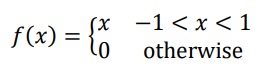
\includegraphics{wiki/q2.jpg}

  \begin{enumerate}
  \def\labelenumii{\arabic{enumii}.}
  \setcounter{enumii}{1}
  \tightlist
  \item
    Plot gained estimated function.
  \end{enumerate}
\item
  Do the following tasks on discrete signal
  \texttt{x\ =\ {[}1\ 2\ 3\ 4\ 5\ 0\ 8\ 8{]}} using Haar wavelet:

  \begin{enumerate}
  \def\labelenumii{\arabic{enumii}.}
  \tightlist
  \item
    Decompose into \texttt{V(j)\ =\ V(j-1)\ ⊕\ W(j-1)}
  \item
    Decompose \texttt{W(j-1)} into \texttt{V} and \texttt{W} again
    \texttt{V(j)\ =\ V(j-2)\ ⊕\ W(j-2)\ ⊕\ W(j-1)}
  \item
    Do step 1 and 2 using available \texttt{dwt} functions.
  \end{enumerate}
\item
  The noisy version of \texttt{img1} is \texttt{img2}. Use available
  \texttt{dwt} functions to denoise image using following procedures and
  compare results using \emph{\textbf{PSNR}} metric:

  \begin{enumerate}
  \def\labelenumii{\arabic{enumii}.}
  \tightlist
  \item
    Decompose image one level and remove \texttt{W\_D(j-1)} completely.
  \item
    Decompose image one level and remove \texttt{W\_D(j-1)},
    \texttt{W\_V(j-1)}, and \texttt{W\_H(j-1)} completely.
  \item
    Compare different wavelet function for step 1 and 2.
  \item
    Zeroing all details lead to a low-quality image such as loosing
    edges which are not noises, so it it appropriate to only remove
    details which pertain noises. Propose a method to remove noises
    without hurting details regarding the original image. You are
    allowed to use results demonstrated in papers.
  \item
    Demonstrate your proposed approach via graph,tables, etc.
  \end{enumerate}
\end{enumerate}

    \hypertarget{explain-the-differences-between-dct-and-wavelet}{%
\subsection{1 Explain the differences between DCT and
Wavelet}\label{explain-the-differences-between-dct-and-wavelet}}

\begin{enumerate}
\def\labelenumi{\arabic{enumi}.}
\item
  First point I would like to focus on is that transforms like DCT or
  DFT work globally, but DWT has localization feature which mean we can
  play with coefficients in the way that only affect a particular
  spatial characteristic of the image, for instance, in DCT a particular
  cosine value is for all matched characterestics in whole image that if
  we zero it, we lose that feature in entire image.
\item
  The second feature of wavelets is that they perform scalable analysis
  on the signal which means every signal can be constructed using
  different scales and position of the basis functions, for instance,
  very large wavelets can represent coarse feature while small wavelets
  can represent very fine details.
\item
  Using DWT, we can approximate a function with a few coefficients in
  comparison with DCT which is absolutely useful in image comparission
  where it is currently is being used in JPEG2000.
\item
  As explained in the first point, because of localization feature,
  almost images can be compressed without considerable degradation.
\end{enumerate}

    \hypertarget{using-available-formulas-in-the-book}{%
\subsection{2 Using available formulas in the
book:}\label{using-available-formulas-in-the-book}}

\begin{enumerate}
\def\labelenumi{\arabic{enumi}.}
\tightlist
\item
  calculate \texttt{c0}, \texttt{d0}, and \texttt{d1} coefficient for
  Haar wavelet.
\end{enumerate}

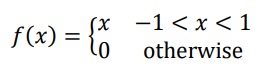
\includegraphics{wiki/q2.jpg} 2. Plot gained estimated function for
\texttt{f(x)}.

    \hypertarget{a}{%
\subsubsection{2.A}\label{a}}

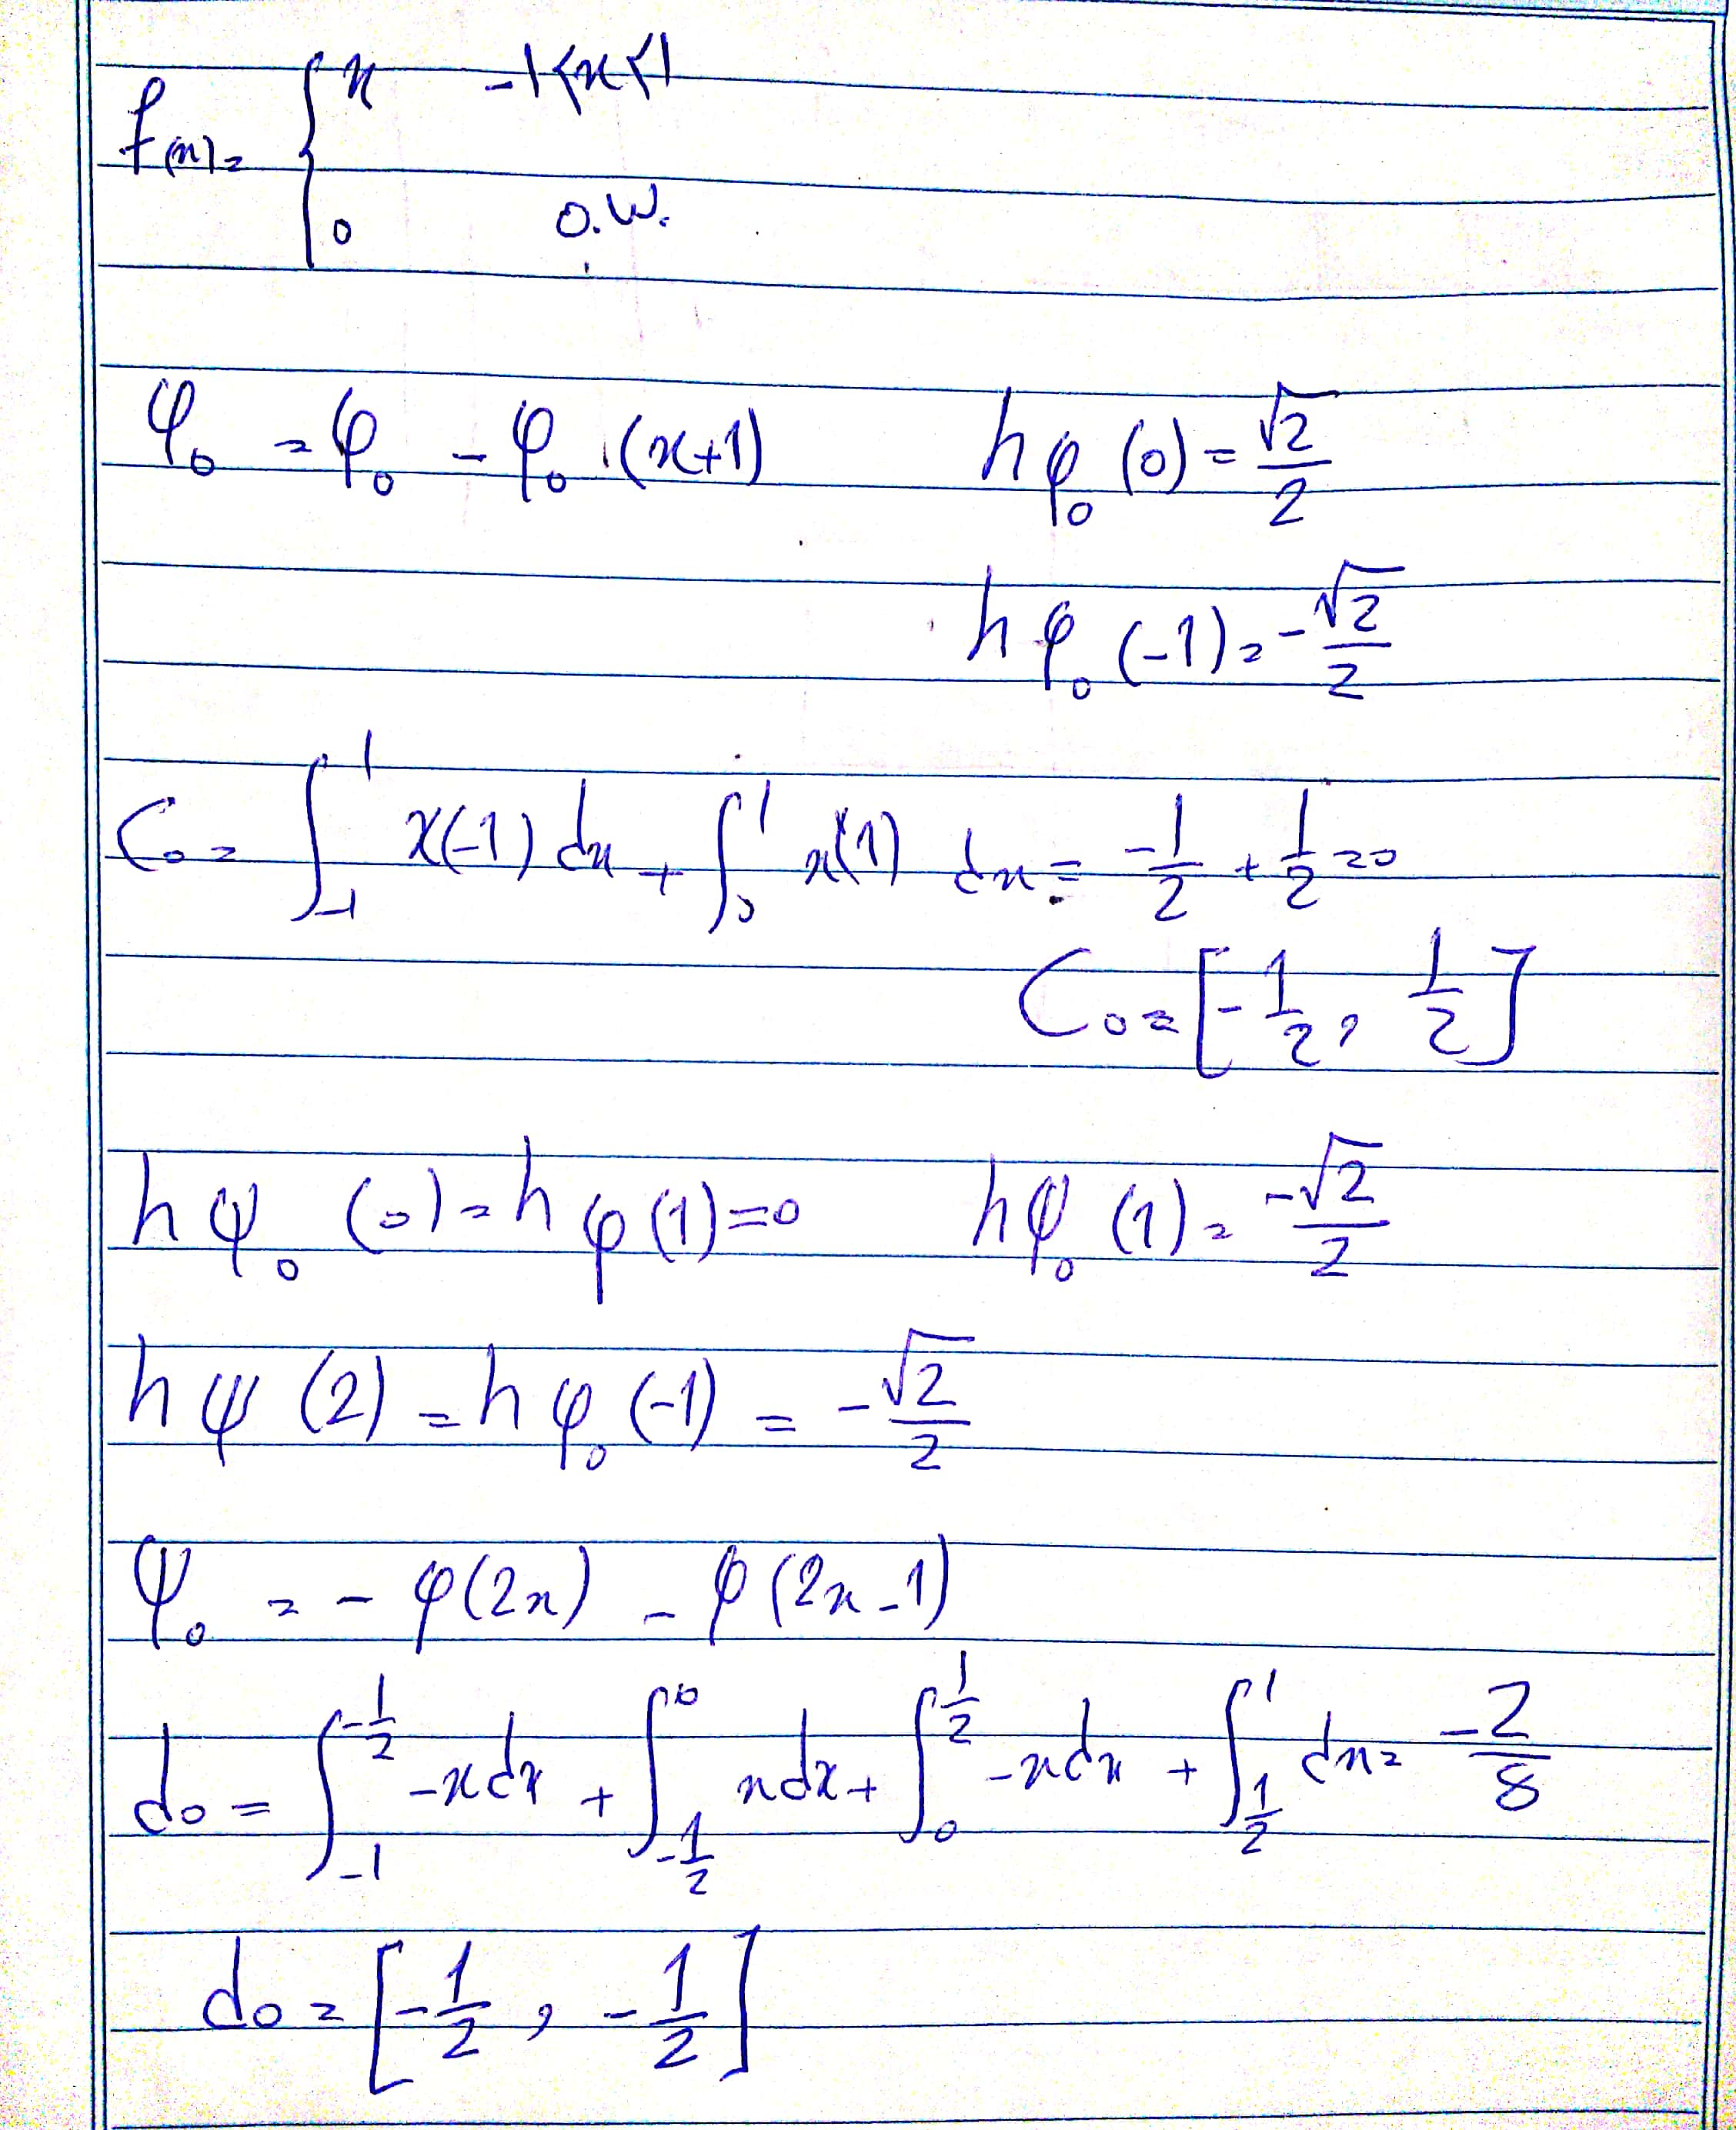
\includegraphics{wiki/eqq2.jpg}

    \hypertarget{b}{%
\subsubsection{2.B}\label{b}}

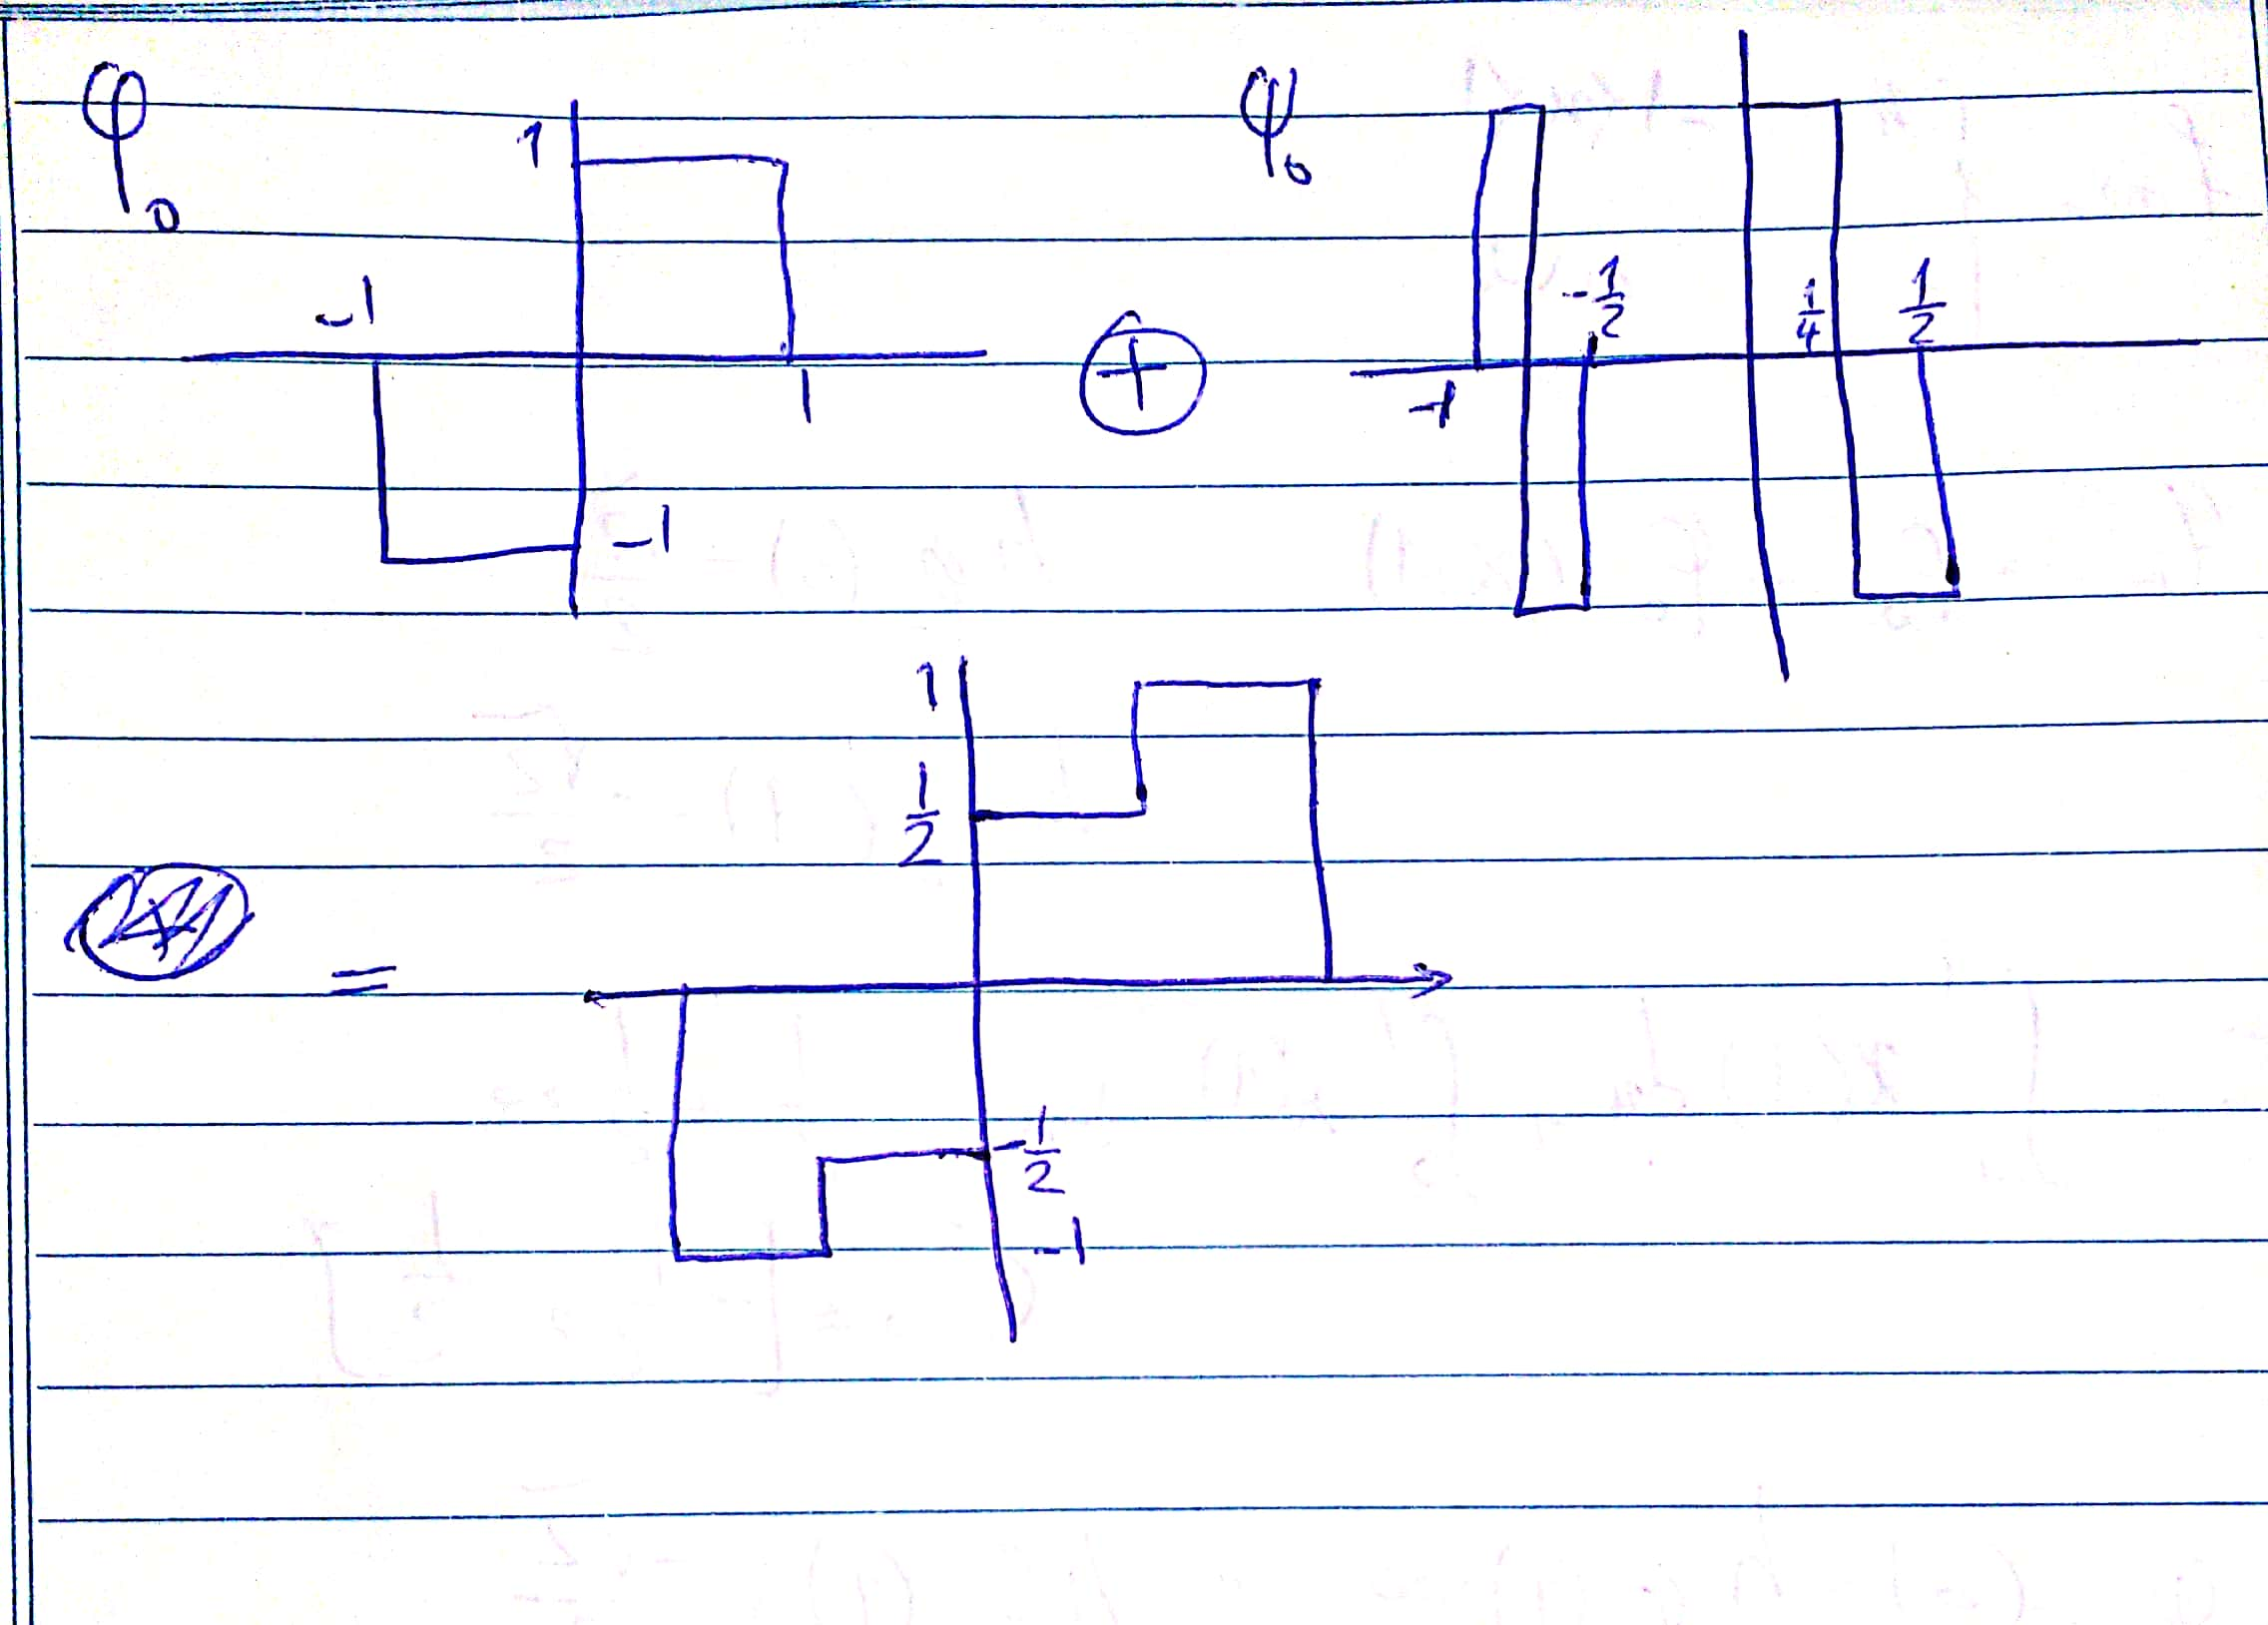
\includegraphics{wiki/graph_q2.jpg}

    \hypertarget{do-the-following-tasks-on-discrete-signal-x-1-2-3-4-5-0-8-8-using-haar-wavelet}{%
\subsection{\texorpdfstring{3 Do the following tasks on discrete signal
\texttt{x\ =\ {[}1\ 2\ 3\ 4\ 5\ 0\ 8\ 8{]}} using Haar
wavelet:}{3 Do the following tasks on discrete signal x = {[}1 2 3 4 5 0 8 8{]} using Haar wavelet:}}\label{do-the-following-tasks-on-discrete-signal-x-1-2-3-4-5-0-8-8-using-haar-wavelet}}

\begin{enumerate}
\def\labelenumi{\arabic{enumi}.}
\tightlist
\item
  Decompose into \texttt{V(j)\ =\ V(j-1)\ ⊕\ W(j-1)}
\item
  Decompose \texttt{W(j-1)} into \texttt{V} and \texttt{W} again
  \texttt{V(j)\ =\ V(j-2)\ ⊕\ W(j-2)\ ⊕\ W(j-1)}
\item
  Do step 1 and 2 using available \texttt{dwt} functions.
\end{enumerate}

    \begin{Verbatim}[commandchars=\\\{\}]
{\color{incolor}In [{\color{incolor}105}]:} \PY{k+kn}{import} \PY{n+nn}{pywt}
          \PY{k+kn}{from} \PY{n+nn}{pywt} \PY{k}{import} \PY{n}{wavedec}
          \PY{k+kn}{import} \PY{n+nn}{numpy} \PY{k}{as} \PY{n+nn}{np}
\end{Verbatim}


    \hypertarget{a-decompose-into-vj-vj-1-wj-1}{%
\paragraph{3.A Decompose into V(j) = V(j-1) ⊕
W(j-1)}\label{a-decompose-into-vj-vj-1-wj-1}}

First of all, based on the book, we only need \texttt{phi(0,0)} and
\texttt{psi(0,0)} to calculate \texttt{V(0)} but I do not know how this
library return those values. It is obvious that \texttt{phi(0,0)} is an
array of all \texttt{1}, so the result should be consistent if we do not
take wavelet of the approximation part. So I cannot handle this question
if I am going to validate my answers using this library. I could not
find any usefull examples in the book, internet etc! Here is the formula
in the book, and it says the first value is consistent in any level. But
the library only return this value at maximum possible level of wavelet,
not any lower. 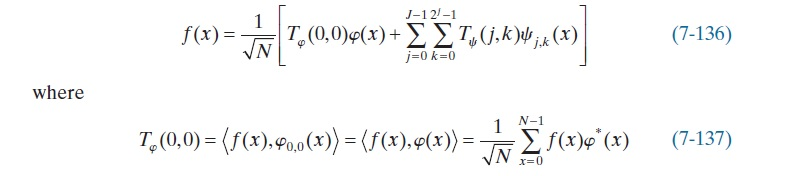
\includegraphics{wiki/dwt0.jpg}

And here is an example in the book compared results using library.

    \begin{Verbatim}[commandchars=\\\{\}]
{\color{incolor}In [{\color{incolor}110}]:} \PY{n}{x} \PY{o}{=} \PY{p}{[}\PY{l+m+mi}{1}\PY{p}{,} \PY{l+m+mi}{4}\PY{p}{,} \PY{o}{\PYZhy{}}\PY{l+m+mi}{3}\PY{p}{,} \PY{l+m+mi}{0}\PY{p}{]}
          \PY{n+nb}{print}\PY{p}{(}\PY{n}{wavedec}\PY{p}{(}\PY{n}{x}\PY{p}{,} \PY{l+s+s1}{\PYZsq{}}\PY{l+s+s1}{haar}\PY{l+s+s1}{\PYZsq{}}\PY{p}{,} \PY{n}{mode}\PY{o}{=}\PY{l+s+s1}{\PYZsq{}}\PY{l+s+s1}{zero}\PY{l+s+s1}{\PYZsq{}}\PY{p}{,} \PY{n}{level}\PY{o}{=}\PY{l+m+mi}{1}\PY{p}{)}\PY{p}{)}
          \PY{n+nb}{print}\PY{p}{(}\PY{n}{np}\PY{o}{.}\PY{n}{array}\PY{p}{(}\PY{n}{x}\PY{p}{)}\PY{n+nd}{@np}\PY{o}{.}\PY{n}{array}\PY{p}{(}\PY{p}{[}\PY{l+m+mi}{1}\PY{p}{,}\PY{l+m+mi}{1}\PY{p}{,}\PY{l+m+mi}{1}\PY{p}{,}\PY{l+m+mi}{1}\PY{p}{]}\PY{p}{)}\PY{o}{/}\PY{l+m+mi}{2}\PY{p}{)}
          \PY{n+nb}{print}\PY{p}{(}\PY{n}{wavedec}\PY{p}{(}\PY{n}{x}\PY{p}{,} \PY{l+s+s1}{\PYZsq{}}\PY{l+s+s1}{haar}\PY{l+s+s1}{\PYZsq{}}\PY{p}{,} \PY{n}{mode}\PY{o}{=}\PY{l+s+s1}{\PYZsq{}}\PY{l+s+s1}{zero}\PY{l+s+s1}{\PYZsq{}}\PY{p}{,} \PY{n}{level}\PY{o}{=}\PY{l+m+mi}{2}\PY{p}{)}\PY{p}{)}
\end{Verbatim}


    \begin{Verbatim}[commandchars=\\\{\}]
[array([ 3.53553391, -2.12132034]), array([-2.12132034, -2.12132034])]
1.0
[array([ 1.]), array([ 4.]), array([-2.12132034, -2.12132034])]

    \end{Verbatim}

    \hypertarget{section}{%
\section{}\label{section}}

The question in the pdf:

    \begin{Verbatim}[commandchars=\\\{\}]
{\color{incolor}In [{\color{incolor}122}]:} \PY{n}{x} \PY{o}{=} \PY{n}{np}\PY{o}{.}\PY{n}{array}\PY{p}{(}\PY{p}{[}\PY{l+m+mi}{1}\PY{p}{,} \PY{l+m+mi}{2}\PY{p}{,} \PY{l+m+mi}{3}\PY{p}{,} \PY{l+m+mi}{4}\PY{p}{,} \PY{l+m+mi}{5}\PY{p}{,} \PY{l+m+mi}{0}\PY{p}{,} \PY{l+m+mi}{8}\PY{p}{,} \PY{l+m+mi}{8}\PY{p}{]}\PY{p}{)}
          \PY{n+nb}{print}\PY{p}{(}\PY{n}{wavedec}\PY{p}{(}\PY{n}{x}\PY{p}{,} \PY{l+s+s1}{\PYZsq{}}\PY{l+s+s1}{haar}\PY{l+s+s1}{\PYZsq{}}\PY{p}{,} \PY{n}{mode}\PY{o}{=}\PY{l+s+s1}{\PYZsq{}}\PY{l+s+s1}{zero}\PY{l+s+s1}{\PYZsq{}}\PY{p}{)}\PY{p}{)}
\end{Verbatim}


    \begin{Verbatim}[commandchars=\\\{\}]
[array([ 10.96015511]), array([-3.8890873]), array([-2. , -5.5]), array([-0.70710678, -0.70710678,  3.53553391,  0.        ])]

    \end{Verbatim}

    \begin{Verbatim}[commandchars=\\\{\}]
{\color{incolor}In [{\color{incolor}121}]:} \PY{n}{a} \PY{o}{=} \PY{n}{x}\PY{n+nd}{@np}\PY{o}{.}\PY{n}{array}\PY{p}{(}\PY{p}{[}\PY{l+m+mi}{1}\PY{p}{,}\PY{l+m+mi}{1}\PY{p}{,}\PY{l+m+mi}{1}\PY{p}{,}\PY{l+m+mi}{1}\PY{p}{,}\PY{l+m+mi}{1}\PY{p}{,}\PY{l+m+mi}{1}\PY{p}{,}\PY{l+m+mi}{1}\PY{p}{,}\PY{l+m+mi}{1}\PY{p}{]}\PY{p}{)}\PY{o}{/}\PY{l+m+mi}{3}
          \PY{n}{d0} \PY{o}{=} \PY{n}{x}\PY{n+nd}{@np}\PY{o}{.}\PY{n}{array}\PY{p}{(}\PY{p}{[}\PY{l+m+mi}{1}\PY{p}{,}\PY{l+m+mi}{1}\PY{p}{,}\PY{l+m+mi}{1}\PY{p}{,}\PY{l+m+mi}{1}\PY{p}{,}\PY{o}{\PYZhy{}}\PY{l+m+mi}{1}\PY{p}{,}\PY{o}{\PYZhy{}}\PY{l+m+mi}{1}\PY{p}{,}\PY{o}{\PYZhy{}}\PY{l+m+mi}{1}\PY{p}{,}\PY{o}{\PYZhy{}}\PY{l+m+mi}{1}\PY{p}{]}\PY{p}{)}\PY{o}{/}\PY{l+m+mi}{3}
          \PY{n}{d1} \PY{o}{=} \PY{n}{x}\PY{n+nd}{@np}\PY{o}{.}\PY{n}{array}\PY{p}{(}\PY{p}{[}\PY{n}{np}\PY{o}{.}\PY{n}{sqrt}\PY{p}{(}\PY{l+m+mi}{2}\PY{p}{)}\PY{p}{,}\PY{n}{np}\PY{o}{.}\PY{n}{sqrt}\PY{p}{(}\PY{l+m+mi}{2}\PY{p}{)}\PY{p}{,}\PY{o}{\PYZhy{}}\PY{n}{np}\PY{o}{.}\PY{n}{sqrt}\PY{p}{(}\PY{l+m+mi}{2}\PY{p}{)}\PY{p}{,}\PY{o}{\PYZhy{}}\PY{n}{np}\PY{o}{.}\PY{n}{sqrt}\PY{p}{(}\PY{l+m+mi}{2}\PY{p}{)}\PY{p}{,}\PY{l+m+mi}{0}\PY{p}{,}\PY{l+m+mi}{0}\PY{p}{,}\PY{l+m+mi}{0}\PY{p}{,}\PY{l+m+mi}{0}\PY{p}{]}\PY{p}{)}\PY{o}{/}\PY{l+m+mi}{3}
          \PY{n}{d2} \PY{o}{=} \PY{n}{x}\PY{n+nd}{@np}\PY{o}{.}\PY{n}{array}\PY{p}{(}\PY{p}{[}\PY{l+m+mi}{0}\PY{p}{,}\PY{l+m+mi}{0}\PY{p}{,}\PY{l+m+mi}{0}\PY{p}{,}\PY{l+m+mi}{0}\PY{p}{,}\PY{n}{np}\PY{o}{.}\PY{n}{sqrt}\PY{p}{(}\PY{l+m+mi}{2}\PY{p}{)}\PY{p}{,}\PY{n}{np}\PY{o}{.}\PY{n}{sqrt}\PY{p}{(}\PY{l+m+mi}{2}\PY{p}{)}\PY{p}{,}\PY{o}{\PYZhy{}}\PY{n}{np}\PY{o}{.}\PY{n}{sqrt}\PY{p}{(}\PY{l+m+mi}{2}\PY{p}{)}\PY{p}{,}\PY{o}{\PYZhy{}}\PY{n}{np}\PY{o}{.}\PY{n}{sqrt}\PY{p}{(}\PY{l+m+mi}{2}\PY{p}{)}\PY{p}{]}\PY{p}{)}\PY{o}{/}\PY{l+m+mi}{3}
          \PY{n+nb}{print}\PY{p}{(}\PY{n}{a}\PY{p}{,} \PY{n}{d0}\PY{p}{,} \PY{n}{d1}\PY{p}{,} \PY{n}{d2}\PY{p}{)}
\end{Verbatim}


    \begin{Verbatim}[commandchars=\\\{\}]
10.3333333333 -3.66666666667 -1.88561808316 -5.1854497287

    \end{Verbatim}

    \hypertarget{c-do-step-1-and-2-using-available-dwt-functions}{%
\paragraph{\texorpdfstring{3.C Do Step 1 and 2 Using Available
\texttt{DWT}
Functions}{3.C Do Step 1 and 2 Using Available DWT Functions}}\label{c-do-step-1-and-2-using-available-dwt-functions}}

    \begin{Verbatim}[commandchars=\\\{\}]
{\color{incolor}In [{\color{incolor}131}]:} \PY{n}{wavedec}\PY{p}{(}\PY{n}{x}\PY{p}{,} \PY{l+s+s1}{\PYZsq{}}\PY{l+s+s1}{haar}\PY{l+s+s1}{\PYZsq{}}\PY{p}{,} \PY{n}{mode}\PY{o}{=}\PY{l+s+s1}{\PYZsq{}}\PY{l+s+s1}{zero}\PY{l+s+s1}{\PYZsq{}}\PY{p}{,} \PY{n}{level}\PY{o}{=}\PY{l+m+mi}{1}\PY{p}{)}
\end{Verbatim}


\begin{Verbatim}[commandchars=\\\{\}]
{\color{outcolor}Out[{\color{outcolor}131}]:} [array([  2.12132034,   4.94974747,   3.53553391,  11.3137085 ]),
           array([-0.70710678, -0.70710678,  3.53553391,  0.        ])]
\end{Verbatim}
            
    \begin{Verbatim}[commandchars=\\\{\}]
{\color{incolor}In [{\color{incolor}144}]:} \PY{n}{wavedec}\PY{p}{(}\PY{n}{wavedec}\PY{p}{(}\PY{n}{x}\PY{p}{,} \PY{l+s+s1}{\PYZsq{}}\PY{l+s+s1}{haar}\PY{l+s+s1}{\PYZsq{}}\PY{p}{,} \PY{n}{mode}\PY{o}{=}\PY{l+s+s1}{\PYZsq{}}\PY{l+s+s1}{zero}\PY{l+s+s1}{\PYZsq{}}\PY{p}{,} \PY{n}{level}\PY{o}{=}\PY{l+m+mi}{1}\PY{p}{)}\PY{p}{[}\PY{l+m+mi}{1}\PY{p}{]}\PY{p}{,} \PY{l+s+s1}{\PYZsq{}}\PY{l+s+s1}{haar}\PY{l+s+s1}{\PYZsq{}}\PY{p}{,} \PY{n}{mode}\PY{o}{=}\PY{l+s+s1}{\PYZsq{}}\PY{l+s+s1}{zero}\PY{l+s+s1}{\PYZsq{}}\PY{p}{,} \PY{n}{level} \PY{o}{=}\PY{l+m+mi}{1}\PY{p}{)}
\end{Verbatim}


\begin{Verbatim}[commandchars=\\\{\}]
{\color{outcolor}Out[{\color{outcolor}144}]:} [array([-1. ,  2.5]), array([ -1.11022302e-16,   2.50000000e+00])]
\end{Verbatim}
            
    \hypertarget{the-noisy-version-of-img1-is-img2.-use-available-dwt-functions-to-denoise-image-using-following-procedures-and-compare-results-using-psnr-metric}{%
\subsection{\texorpdfstring{4 The noisy version of \texttt{img1} is
\texttt{img2}. Use available \texttt{dwt} functions to denoise image
using following procedures and compare results using
\emph{\textbf{PSNR}}
metric:}{4 The noisy version of img1 is img2. Use available dwt functions to denoise image using following procedures and compare results using PSNR metric:}}\label{the-noisy-version-of-img1-is-img2.-use-available-dwt-functions-to-denoise-image-using-following-procedures-and-compare-results-using-psnr-metric}}

\begin{enumerate}
\def\labelenumi{\arabic{enumi}.}
\tightlist
\item
  Decompose image one level and remove \texttt{W\_D(j-1)} completely.
\item
  Decompose image one level and remove \texttt{W\_D(j-1)},
  \texttt{W\_V(j-1)}, and \texttt{W\_H(j-1)} completely.
\item
  Compare different wavelet function for step 1 and 2.
\item
  Zeroing all details lead to a low-quality image such as loosing edges
  which are not noises, so it it appropriate to only remove details
  which pertain noises. Propose a method to remove noises without
  hurting details regarding the original image. You are allowed to use
  results demonstrated in papers.
\item
  Demonstrate your proposed approach via graph,tables, etc.
\end{enumerate}

Here are the images:

\texttt{img1} \includegraphics{img1.bmp} \texttt{img2}
\includegraphics{img2.bmp}

    \begin{Verbatim}[commandchars=\\\{\}]
{\color{incolor}In [{\color{incolor}152}]:} \PY{k+kn}{import} \PY{n+nn}{matplotlib}\PY{n+nn}{.}\PY{n+nn}{pyplot} \PY{k}{as} \PY{n+nn}{plt}
          \PY{k+kn}{from} \PY{n+nn}{skimage}\PY{n+nn}{.}\PY{n+nn}{measure} \PY{k}{import} \PY{n}{compare\PYZus{}psnr}
\end{Verbatim}


    \hypertarget{a-decompose-image-one-level-and-remove-w_dj-1-completely.}{%
\paragraph{4.A Decompose image one level and remove W\_D(j-1)
completely.}\label{a-decompose-image-one-level-and-remove-w_dj-1-completely.}}

    \begin{Verbatim}[commandchars=\\\{\}]
{\color{incolor}In [{\color{incolor}166}]:} \PY{n}{noisy} \PY{o}{=} \PY{n}{plt}\PY{o}{.}\PY{n}{imread}\PY{p}{(}\PY{l+s+s1}{\PYZsq{}}\PY{l+s+s1}{img2.bmp}\PY{l+s+s1}{\PYZsq{}}\PY{p}{)}
          \PY{n}{original} \PY{o}{=} \PY{n}{plt}\PY{o}{.}\PY{n}{imread}\PY{p}{(}\PY{l+s+s1}{\PYZsq{}}\PY{l+s+s1}{img1.bmp}\PY{l+s+s1}{\PYZsq{}}\PY{p}{)}
          \PY{c+c1}{\PYZsh{} Wavelet transform of image, and plot approximation and details}
          \PY{n}{titles} \PY{o}{=} \PY{p}{[}\PY{l+s+s1}{\PYZsq{}}\PY{l+s+s1}{Approximation}\PY{l+s+s1}{\PYZsq{}}\PY{p}{,} \PY{l+s+s1}{\PYZsq{}}\PY{l+s+s1}{ Horizontal detail}\PY{l+s+s1}{\PYZsq{}}\PY{p}{,}
                    \PY{l+s+s1}{\PYZsq{}}\PY{l+s+s1}{Vertical detail}\PY{l+s+s1}{\PYZsq{}}\PY{p}{,} \PY{l+s+s1}{\PYZsq{}}\PY{l+s+s1}{Diagonal detail}\PY{l+s+s1}{\PYZsq{}}\PY{p}{]}
          \PY{n}{LL}\PY{p}{,} \PY{p}{(}\PY{n}{LH}\PY{p}{,} \PY{n}{HL}\PY{p}{,} \PY{n}{HH}\PY{p}{)} \PY{o}{=} \PY{n}{pywt}\PY{o}{.}\PY{n}{dwt2}\PY{p}{(}\PY{n}{noisy}\PY{p}{,} \PY{l+s+s1}{\PYZsq{}}\PY{l+s+s1}{haar}\PY{l+s+s1}{\PYZsq{}}\PY{p}{)}
          \PY{n}{fig}\PY{p}{,} \PY{n}{ax} \PY{o}{=} \PY{n}{plt}\PY{o}{.}\PY{n}{subplots}\PY{p}{(}\PY{n}{nrows}\PY{o}{=}\PY{l+m+mi}{1}\PY{p}{,} \PY{n}{ncols}\PY{o}{=}\PY{l+m+mi}{4}\PY{p}{,} \PY{n}{figsize}\PY{o}{=}\PY{p}{(}\PY{l+m+mi}{20}\PY{p}{,} \PY{l+m+mi}{15}\PY{p}{)}\PY{p}{)}
          \PY{k}{for} \PY{n}{i}\PY{p}{,} \PY{n}{a} \PY{o+ow}{in} \PY{n+nb}{enumerate}\PY{p}{(}\PY{p}{[}\PY{n}{LL}\PY{p}{,} \PY{n}{LH}\PY{p}{,} \PY{n}{HL}\PY{p}{,} \PY{n}{HH}\PY{p}{]}\PY{p}{)}\PY{p}{:}
              \PY{n}{ax}\PY{p}{[}\PY{n}{i}\PY{p}{]}\PY{o}{.}\PY{n}{imshow}\PY{p}{(}\PY{n}{a}\PY{p}{,} \PY{n}{cmap}\PY{o}{=}\PY{n}{plt}\PY{o}{.}\PY{n}{cm}\PY{o}{.}\PY{n}{gray}\PY{p}{)}
              \PY{n}{ax}\PY{p}{[}\PY{n}{i}\PY{p}{]}\PY{o}{.}\PY{n}{set\PYZus{}title}\PY{p}{(}\PY{n}{titles}\PY{p}{[}\PY{n}{i}\PY{p}{]}\PY{p}{,} \PY{n}{fontsize}\PY{o}{=}\PY{l+m+mi}{10}\PY{p}{)}
              \PY{n}{ax}\PY{p}{[}\PY{n}{i}\PY{p}{]}\PY{o}{.}\PY{n}{set\PYZus{}xticks}\PY{p}{(}\PY{p}{[}\PY{p}{]}\PY{p}{)}
              \PY{n}{ax}\PY{p}{[}\PY{n}{i}\PY{p}{]}\PY{o}{.}\PY{n}{set\PYZus{}yticks}\PY{p}{(}\PY{p}{[}\PY{p}{]}\PY{p}{)}
          
          \PY{n}{fig}\PY{o}{.}\PY{n}{tight\PYZus{}layout}\PY{p}{(}\PY{p}{)}
          \PY{n}{plt}\PY{o}{.}\PY{n}{show}\PY{p}{(}\PY{p}{)}
          
          \PY{c+c1}{\PYZsh{} denoising}
          \PY{n}{titles} \PY{o}{=} \PY{p}{[}\PY{l+s+s1}{\PYZsq{}}\PY{l+s+s1}{noisy}\PY{l+s+s1}{\PYZsq{}}\PY{p}{,} \PY{l+s+s1}{\PYZsq{}}\PY{l+s+s1}{denoised}\PY{l+s+s1}{\PYZsq{}}\PY{p}{]}
          \PY{n}{denoised} \PY{o}{=} \PY{n}{pywt}\PY{o}{.}\PY{n}{idwt2}\PY{p}{(}\PY{p}{(}\PY{n}{LL}\PY{p}{,} \PY{p}{(}\PY{n}{LH}\PY{p}{,} \PY{n}{HL}\PY{p}{,} \PY{k+kc}{None}\PY{p}{)}\PY{p}{)}\PY{p}{,} \PY{l+s+s1}{\PYZsq{}}\PY{l+s+s1}{haar}\PY{l+s+s1}{\PYZsq{}}\PY{p}{)}
          \PY{n}{fig}\PY{p}{,} \PY{n}{ax} \PY{o}{=} \PY{n}{plt}\PY{o}{.}\PY{n}{subplots}\PY{p}{(}\PY{n}{nrows}\PY{o}{=}\PY{l+m+mi}{1}\PY{p}{,} \PY{n}{ncols}\PY{o}{=}\PY{l+m+mi}{2}\PY{p}{,} \PY{n}{figsize}\PY{o}{=}\PY{p}{(}\PY{l+m+mi}{15}\PY{p}{,} \PY{l+m+mi}{10}\PY{p}{)}\PY{p}{)}
          \PY{k}{for} \PY{n}{i}\PY{p}{,} \PY{n}{a} \PY{o+ow}{in} \PY{n+nb}{enumerate}\PY{p}{(}\PY{p}{[}\PY{n}{noisy}\PY{p}{,} \PY{n}{denoised}\PY{p}{]}\PY{p}{)}\PY{p}{:}
              \PY{n}{ax}\PY{p}{[}\PY{n}{i}\PY{p}{]}\PY{o}{.}\PY{n}{imshow}\PY{p}{(}\PY{n}{a}\PY{p}{,} \PY{n}{cmap}\PY{o}{=}\PY{n}{plt}\PY{o}{.}\PY{n}{cm}\PY{o}{.}\PY{n}{gray}\PY{p}{)}
              \PY{n}{ax}\PY{p}{[}\PY{n}{i}\PY{p}{]}\PY{o}{.}\PY{n}{set\PYZus{}title}\PY{p}{(}\PY{n}{titles}\PY{p}{[}\PY{n}{i}\PY{p}{]}\PY{p}{,} \PY{n}{fontsize}\PY{o}{=}\PY{l+m+mi}{10}\PY{p}{)}
              \PY{n}{ax}\PY{p}{[}\PY{n}{i}\PY{p}{]}\PY{o}{.}\PY{n}{set\PYZus{}xticks}\PY{p}{(}\PY{p}{[}\PY{p}{]}\PY{p}{)}
              \PY{n}{ax}\PY{p}{[}\PY{n}{i}\PY{p}{]}\PY{o}{.}\PY{n}{set\PYZus{}yticks}\PY{p}{(}\PY{p}{[}\PY{p}{]}\PY{p}{)}
          
          \PY{n}{fig}\PY{o}{.}\PY{n}{tight\PYZus{}layout}\PY{p}{(}\PY{p}{)}
          \PY{n}{plt}\PY{o}{.}\PY{n}{show}\PY{p}{(}\PY{p}{)}
          
          \PY{n+nb}{print}\PY{p}{(}\PY{l+s+s1}{\PYZsq{}}\PY{l+s+s1}{PSNR value: }\PY{l+s+si}{\PYZob{}\PYZcb{}}\PY{l+s+s1}{\PYZsq{}}\PY{o}{.}\PY{n}{format}\PY{p}{(}\PY{n}{compare\PYZus{}psnr}\PY{p}{(}\PY{n}{original}\PY{p}{,} \PY{n}{denoised}\PY{p}{)}\PY{p}{)}\PY{p}{)}
\end{Verbatim}


    \begin{center}
    \adjustimage{max size={0.9\linewidth}{0.9\paperheight}}{output_18_0.png}
    \end{center}
    { \hspace*{\fill} \\}
    
    \begin{center}
    \adjustimage{max size={0.9\linewidth}{0.9\paperheight}}{output_18_1.png}
    \end{center}
    { \hspace*{\fill} \\}
    
    \begin{Verbatim}[commandchars=\\\{\}]
PSNR value: 18.636604880778794

    \end{Verbatim}

    \hypertarget{b-decompose-image-one-level-and-remove-w_dj-1-w_vj-1-and-w_hj-1-completely.}{%
\paragraph{4.B Decompose image one level and remove W\_D(j-1),
W\_V(j-1), and W\_H(j-1)
completely.}\label{b-decompose-image-one-level-and-remove-w_dj-1-w_vj-1-and-w_hj-1-completely.}}

    \begin{Verbatim}[commandchars=\\\{\}]
{\color{incolor}In [{\color{incolor}167}]:} \PY{n}{noisy} \PY{o}{=} \PY{n}{plt}\PY{o}{.}\PY{n}{imread}\PY{p}{(}\PY{l+s+s1}{\PYZsq{}}\PY{l+s+s1}{img2.bmp}\PY{l+s+s1}{\PYZsq{}}\PY{p}{)}
          \PY{n}{original} \PY{o}{=} \PY{n}{plt}\PY{o}{.}\PY{n}{imread}\PY{p}{(}\PY{l+s+s1}{\PYZsq{}}\PY{l+s+s1}{img1.bmp}\PY{l+s+s1}{\PYZsq{}}\PY{p}{)}
          \PY{c+c1}{\PYZsh{} Wavelet transform of image, and plot approximation and details}
          \PY{n}{titles} \PY{o}{=} \PY{p}{[}\PY{l+s+s1}{\PYZsq{}}\PY{l+s+s1}{Approximation}\PY{l+s+s1}{\PYZsq{}}\PY{p}{,} \PY{l+s+s1}{\PYZsq{}}\PY{l+s+s1}{ Horizontal detail}\PY{l+s+s1}{\PYZsq{}}\PY{p}{,}
                    \PY{l+s+s1}{\PYZsq{}}\PY{l+s+s1}{Vertical detail}\PY{l+s+s1}{\PYZsq{}}\PY{p}{,} \PY{l+s+s1}{\PYZsq{}}\PY{l+s+s1}{Diagonal detail}\PY{l+s+s1}{\PYZsq{}}\PY{p}{]}
          \PY{n}{LL}\PY{p}{,} \PY{p}{(}\PY{n}{LH}\PY{p}{,} \PY{n}{HL}\PY{p}{,} \PY{n}{HH}\PY{p}{)} \PY{o}{=} \PY{n}{pywt}\PY{o}{.}\PY{n}{dwt2}\PY{p}{(}\PY{n}{noisy}\PY{p}{,} \PY{l+s+s1}{\PYZsq{}}\PY{l+s+s1}{haar}\PY{l+s+s1}{\PYZsq{}}\PY{p}{)}
          \PY{n}{fig}\PY{p}{,} \PY{n}{ax} \PY{o}{=} \PY{n}{plt}\PY{o}{.}\PY{n}{subplots}\PY{p}{(}\PY{n}{nrows}\PY{o}{=}\PY{l+m+mi}{1}\PY{p}{,} \PY{n}{ncols}\PY{o}{=}\PY{l+m+mi}{4}\PY{p}{,} \PY{n}{figsize}\PY{o}{=}\PY{p}{(}\PY{l+m+mi}{20}\PY{p}{,} \PY{l+m+mi}{15}\PY{p}{)}\PY{p}{)}
          \PY{k}{for} \PY{n}{i}\PY{p}{,} \PY{n}{a} \PY{o+ow}{in} \PY{n+nb}{enumerate}\PY{p}{(}\PY{p}{[}\PY{n}{LL}\PY{p}{,} \PY{n}{LH}\PY{p}{,} \PY{n}{HL}\PY{p}{,} \PY{n}{HH}\PY{p}{]}\PY{p}{)}\PY{p}{:}
              \PY{n}{ax}\PY{p}{[}\PY{n}{i}\PY{p}{]}\PY{o}{.}\PY{n}{imshow}\PY{p}{(}\PY{n}{a}\PY{p}{,} \PY{n}{cmap}\PY{o}{=}\PY{n}{plt}\PY{o}{.}\PY{n}{cm}\PY{o}{.}\PY{n}{gray}\PY{p}{)}
              \PY{n}{ax}\PY{p}{[}\PY{n}{i}\PY{p}{]}\PY{o}{.}\PY{n}{set\PYZus{}title}\PY{p}{(}\PY{n}{titles}\PY{p}{[}\PY{n}{i}\PY{p}{]}\PY{p}{,} \PY{n}{fontsize}\PY{o}{=}\PY{l+m+mi}{10}\PY{p}{)}
              \PY{n}{ax}\PY{p}{[}\PY{n}{i}\PY{p}{]}\PY{o}{.}\PY{n}{set\PYZus{}xticks}\PY{p}{(}\PY{p}{[}\PY{p}{]}\PY{p}{)}
              \PY{n}{ax}\PY{p}{[}\PY{n}{i}\PY{p}{]}\PY{o}{.}\PY{n}{set\PYZus{}yticks}\PY{p}{(}\PY{p}{[}\PY{p}{]}\PY{p}{)}
          
          \PY{n}{fig}\PY{o}{.}\PY{n}{tight\PYZus{}layout}\PY{p}{(}\PY{p}{)}
          \PY{n}{plt}\PY{o}{.}\PY{n}{show}\PY{p}{(}\PY{p}{)}
          
          \PY{c+c1}{\PYZsh{} denoising}
          \PY{n}{titles} \PY{o}{=} \PY{p}{[}\PY{l+s+s1}{\PYZsq{}}\PY{l+s+s1}{noisy}\PY{l+s+s1}{\PYZsq{}}\PY{p}{,} \PY{l+s+s1}{\PYZsq{}}\PY{l+s+s1}{denoised}\PY{l+s+s1}{\PYZsq{}}\PY{p}{]}
          \PY{n}{denoised} \PY{o}{=} \PY{n}{pywt}\PY{o}{.}\PY{n}{idwt2}\PY{p}{(}\PY{p}{(}\PY{n}{LL}\PY{p}{,} \PY{p}{(}\PY{k+kc}{None}\PY{p}{,} \PY{k+kc}{None}\PY{p}{,} \PY{k+kc}{None}\PY{p}{)}\PY{p}{)}\PY{p}{,} \PY{l+s+s1}{\PYZsq{}}\PY{l+s+s1}{haar}\PY{l+s+s1}{\PYZsq{}}\PY{p}{)}
          \PY{n}{fig}\PY{p}{,} \PY{n}{ax} \PY{o}{=} \PY{n}{plt}\PY{o}{.}\PY{n}{subplots}\PY{p}{(}\PY{n}{nrows}\PY{o}{=}\PY{l+m+mi}{1}\PY{p}{,} \PY{n}{ncols}\PY{o}{=}\PY{l+m+mi}{2}\PY{p}{,} \PY{n}{figsize}\PY{o}{=}\PY{p}{(}\PY{l+m+mi}{15}\PY{p}{,} \PY{l+m+mi}{10}\PY{p}{)}\PY{p}{)}
          \PY{k}{for} \PY{n}{i}\PY{p}{,} \PY{n}{a} \PY{o+ow}{in} \PY{n+nb}{enumerate}\PY{p}{(}\PY{p}{[}\PY{n}{noisy}\PY{p}{,} \PY{n}{denoised}\PY{p}{]}\PY{p}{)}\PY{p}{:}
              \PY{n}{ax}\PY{p}{[}\PY{n}{i}\PY{p}{]}\PY{o}{.}\PY{n}{imshow}\PY{p}{(}\PY{n}{a}\PY{p}{,} \PY{n}{cmap}\PY{o}{=}\PY{n}{plt}\PY{o}{.}\PY{n}{cm}\PY{o}{.}\PY{n}{gray}\PY{p}{)}
              \PY{n}{ax}\PY{p}{[}\PY{n}{i}\PY{p}{]}\PY{o}{.}\PY{n}{set\PYZus{}title}\PY{p}{(}\PY{n}{titles}\PY{p}{[}\PY{n}{i}\PY{p}{]}\PY{p}{,} \PY{n}{fontsize}\PY{o}{=}\PY{l+m+mi}{10}\PY{p}{)}
              \PY{n}{ax}\PY{p}{[}\PY{n}{i}\PY{p}{]}\PY{o}{.}\PY{n}{set\PYZus{}xticks}\PY{p}{(}\PY{p}{[}\PY{p}{]}\PY{p}{)}
              \PY{n}{ax}\PY{p}{[}\PY{n}{i}\PY{p}{]}\PY{o}{.}\PY{n}{set\PYZus{}yticks}\PY{p}{(}\PY{p}{[}\PY{p}{]}\PY{p}{)}
          
          \PY{n}{fig}\PY{o}{.}\PY{n}{tight\PYZus{}layout}\PY{p}{(}\PY{p}{)}
          \PY{n}{plt}\PY{o}{.}\PY{n}{show}\PY{p}{(}\PY{p}{)}
          
          \PY{n+nb}{print}\PY{p}{(}\PY{l+s+s1}{\PYZsq{}}\PY{l+s+s1}{PSNR value: }\PY{l+s+si}{\PYZob{}\PYZcb{}}\PY{l+s+s1}{\PYZsq{}}\PY{o}{.}\PY{n}{format}\PY{p}{(}\PY{n}{compare\PYZus{}psnr}\PY{p}{(}\PY{n}{original}\PY{p}{,} \PY{n}{denoised}\PY{p}{)}\PY{p}{)}\PY{p}{)}
\end{Verbatim}


    \begin{center}
    \adjustimage{max size={0.9\linewidth}{0.9\paperheight}}{output_20_0.png}
    \end{center}
    { \hspace*{\fill} \\}
    
    \begin{center}
    \adjustimage{max size={0.9\linewidth}{0.9\paperheight}}{output_20_1.png}
    \end{center}
    { \hspace*{\fill} \\}
    
    \begin{Verbatim}[commandchars=\\\{\}]
PSNR value: 21.304527635133958

    \end{Verbatim}

    \hypertarget{c-compare-different-wavelet-function-for-step-1-and-2.}{%
\paragraph{4.C Compare different wavelet function for step 1 and
2.}\label{c-compare-different-wavelet-function-for-step-1-and-2.}}

    \begin{Verbatim}[commandchars=\\\{\}]
{\color{incolor}In [{\color{incolor}186}]:} \PY{n}{noisy} \PY{o}{=} \PY{n}{plt}\PY{o}{.}\PY{n}{imread}\PY{p}{(}\PY{l+s+s1}{\PYZsq{}}\PY{l+s+s1}{img2.bmp}\PY{l+s+s1}{\PYZsq{}}\PY{p}{)}
          \PY{n}{original} \PY{o}{=} \PY{n}{plt}\PY{o}{.}\PY{n}{imread}\PY{p}{(}\PY{l+s+s1}{\PYZsq{}}\PY{l+s+s1}{img1.bmp}\PY{l+s+s1}{\PYZsq{}}\PY{p}{)}
          
          \PY{n}{max\PYZus{}hh} \PY{o}{=} \PY{l+m+mi}{0}
          \PY{n}{wave\PYZus{}hh} \PY{o}{=} \PY{l+s+s1}{\PYZsq{}}\PY{l+s+s1}{\PYZsq{}}
          \PY{n}{max\PYZus{}ll} \PY{o}{=} \PY{l+m+mi}{0}
          \PY{n}{wave\PYZus{}ll} \PY{o}{=} \PY{l+s+s1}{\PYZsq{}}\PY{l+s+s1}{\PYZsq{}}
          \PY{k}{for} \PY{n}{family} \PY{o+ow}{in} \PY{n}{pywt}\PY{o}{.}\PY{n}{families}\PY{p}{(}\PY{p}{)}\PY{p}{[}\PY{p}{:}\PY{o}{\PYZhy{}}\PY{l+m+mi}{7}\PY{p}{]}\PY{p}{:}
              \PY{k}{for} \PY{n}{wave} \PY{o+ow}{in} \PY{n}{pywt}\PY{o}{.}\PY{n}{wavelist}\PY{p}{(}\PY{n}{family}\PY{p}{)}\PY{p}{:}
                  \PY{c+c1}{\PYZsh{} Wavelet}
                  \PY{n}{LL}\PY{p}{,} \PY{p}{(}\PY{n}{LH}\PY{p}{,} \PY{n}{HL}\PY{p}{,} \PY{n}{HH}\PY{p}{)} \PY{o}{=} \PY{n}{pywt}\PY{o}{.}\PY{n}{dwt2}\PY{p}{(}\PY{n}{noisy}\PY{p}{,} \PY{n}{wave}\PY{p}{)}
                  \PY{c+c1}{\PYZsh{} denoising}
                  \PY{n}{denoised\PYZus{}HH} \PY{o}{=} \PY{n}{pywt}\PY{o}{.}\PY{n}{idwt2}\PY{p}{(}\PY{p}{(}\PY{n}{LL}\PY{p}{,} \PY{p}{(}\PY{n}{LH}\PY{p}{,} \PY{n}{HL}\PY{p}{,} \PY{k+kc}{None}\PY{p}{)}\PY{p}{)}\PY{p}{,} \PY{n}{wave}\PY{p}{)}
                  \PY{n}{denoised\PYZus{}LL} \PY{o}{=} \PY{n}{pywt}\PY{o}{.}\PY{n}{idwt2}\PY{p}{(}\PY{p}{(}\PY{n}{LL}\PY{p}{,} \PY{p}{(}\PY{k+kc}{None}\PY{p}{,} \PY{k+kc}{None}\PY{p}{,} \PY{k+kc}{None}\PY{p}{)}\PY{p}{)}\PY{p}{,} \PY{n}{wave}\PY{p}{)}
                  \PY{n}{psnr\PYZus{}hh} \PY{o}{=} \PY{n}{compare\PYZus{}psnr}\PY{p}{(}\PY{n}{original}\PY{p}{,} \PY{n}{denoised\PYZus{}HH}\PY{p}{)}
                  \PY{n}{psnr\PYZus{}ll} \PY{o}{=} \PY{n}{compare\PYZus{}psnr}\PY{p}{(}\PY{n}{original}\PY{p}{,} \PY{n}{denoised\PYZus{}LL}\PY{p}{)}
                  \PY{k}{if} \PY{n}{psnr\PYZus{}hh} \PY{o}{\PYZgt{}} \PY{n}{max\PYZus{}hh}\PY{p}{:}
                      \PY{n}{max\PYZus{}hh} \PY{o}{=} \PY{n}{psnr\PYZus{}hh}
                      \PY{n}{wave\PYZus{}hh} \PY{o}{=} \PY{n}{wave}
                  \PY{k}{if} \PY{n}{psnr\PYZus{}ll} \PY{o}{\PYZgt{}} \PY{n}{max\PYZus{}ll}\PY{p}{:}
                      \PY{n}{max\PYZus{}ll} \PY{o}{=} \PY{n}{psnr\PYZus{}ll}
                      \PY{n}{wave\PYZus{}ll} \PY{o}{=} \PY{n}{wave}
          \PY{n+nb}{print}\PY{p}{(}\PY{l+s+s1}{\PYZsq{}}\PY{l+s+s1}{PSNR \PYZhy{} No Diagonal \PYZhy{} wavelet:}\PY{l+s+si}{\PYZob{}\PYZcb{}}\PY{l+s+s1}{ ======\PYZgt{} }\PY{l+s+si}{\PYZob{}\PYZcb{}}\PY{l+s+s1}{\PYZsq{}}\PY{o}{.}\PY{n}{format}\PY{p}{(}\PY{n}{wave\PYZus{}hh}\PY{p}{,} \PY{n}{max\PYZus{}hh}\PY{p}{)}\PY{p}{)}
          \PY{n+nb}{print}\PY{p}{(}\PY{l+s+s1}{\PYZsq{}}\PY{l+s+s1}{PSNR \PYZhy{} Only Approximation \PYZhy{} wavelet:}\PY{l+s+si}{\PYZob{}\PYZcb{}}\PY{l+s+s1}{ ======\PYZgt{} }\PY{l+s+si}{\PYZob{}\PYZcb{}}\PY{l+s+s1}{\PYZsq{}}\PY{o}{.}\PY{n}{format}\PY{p}{(}\PY{n}{wave\PYZus{}ll}\PY{p}{,} \PY{n}{max\PYZus{}ll}\PY{p}{)}\PY{p}{)}
\end{Verbatim}


    \begin{Verbatim}[commandchars=\\\{\}]
PSNR - No Diagonal - wavelet:sym17 ======> 18.67134414690018
PSNR - Only Approximation - wavelet:db32 ======> 21.940123937910926

    \end{Verbatim}

    \begin{Verbatim}[commandchars=\\\{\}]
{\color{incolor}In [{\color{incolor}188}]:} \PY{n}{noisy} \PY{o}{=} \PY{n}{plt}\PY{o}{.}\PY{n}{imread}\PY{p}{(}\PY{l+s+s1}{\PYZsq{}}\PY{l+s+s1}{img2.bmp}\PY{l+s+s1}{\PYZsq{}}\PY{p}{)}
          \PY{n}{original} \PY{o}{=} \PY{n}{plt}\PY{o}{.}\PY{n}{imread}\PY{p}{(}\PY{l+s+s1}{\PYZsq{}}\PY{l+s+s1}{img1.bmp}\PY{l+s+s1}{\PYZsq{}}\PY{p}{)}
          \PY{c+c1}{\PYZsh{} Wavelet transform of image, and plot approximation and details}
          \PY{n}{titles} \PY{o}{=} \PY{p}{[}\PY{l+s+s1}{\PYZsq{}}\PY{l+s+s1}{Approximation}\PY{l+s+s1}{\PYZsq{}}\PY{p}{,} \PY{l+s+s1}{\PYZsq{}}\PY{l+s+s1}{ Horizontal detail}\PY{l+s+s1}{\PYZsq{}}\PY{p}{,}
                    \PY{l+s+s1}{\PYZsq{}}\PY{l+s+s1}{Vertical detail}\PY{l+s+s1}{\PYZsq{}}\PY{p}{,} \PY{l+s+s1}{\PYZsq{}}\PY{l+s+s1}{Diagonal detail}\PY{l+s+s1}{\PYZsq{}}\PY{p}{]}
          \PY{n}{LL}\PY{p}{,} \PY{p}{(}\PY{n}{LH}\PY{p}{,} \PY{n}{HL}\PY{p}{,} \PY{n}{HH}\PY{p}{)} \PY{o}{=} \PY{n}{pywt}\PY{o}{.}\PY{n}{dwt2}\PY{p}{(}\PY{n}{noisy}\PY{p}{,} \PY{l+s+s1}{\PYZsq{}}\PY{l+s+s1}{sym17}\PY{l+s+s1}{\PYZsq{}}\PY{p}{)}
          \PY{n}{fig}\PY{p}{,} \PY{n}{ax} \PY{o}{=} \PY{n}{plt}\PY{o}{.}\PY{n}{subplots}\PY{p}{(}\PY{n}{nrows}\PY{o}{=}\PY{l+m+mi}{1}\PY{p}{,} \PY{n}{ncols}\PY{o}{=}\PY{l+m+mi}{4}\PY{p}{,} \PY{n}{figsize}\PY{o}{=}\PY{p}{(}\PY{l+m+mi}{20}\PY{p}{,} \PY{l+m+mi}{15}\PY{p}{)}\PY{p}{)}
          \PY{k}{for} \PY{n}{i}\PY{p}{,} \PY{n}{a} \PY{o+ow}{in} \PY{n+nb}{enumerate}\PY{p}{(}\PY{p}{[}\PY{n}{LL}\PY{p}{,} \PY{n}{LH}\PY{p}{,} \PY{n}{HL}\PY{p}{,} \PY{n}{HH}\PY{p}{]}\PY{p}{)}\PY{p}{:}
              \PY{n}{ax}\PY{p}{[}\PY{n}{i}\PY{p}{]}\PY{o}{.}\PY{n}{imshow}\PY{p}{(}\PY{n}{a}\PY{p}{,} \PY{n}{cmap}\PY{o}{=}\PY{n}{plt}\PY{o}{.}\PY{n}{cm}\PY{o}{.}\PY{n}{gray}\PY{p}{)}
              \PY{n}{ax}\PY{p}{[}\PY{n}{i}\PY{p}{]}\PY{o}{.}\PY{n}{set\PYZus{}title}\PY{p}{(}\PY{n}{titles}\PY{p}{[}\PY{n}{i}\PY{p}{]}\PY{p}{,} \PY{n}{fontsize}\PY{o}{=}\PY{l+m+mi}{10}\PY{p}{)}
              \PY{n}{ax}\PY{p}{[}\PY{n}{i}\PY{p}{]}\PY{o}{.}\PY{n}{set\PYZus{}xticks}\PY{p}{(}\PY{p}{[}\PY{p}{]}\PY{p}{)}
              \PY{n}{ax}\PY{p}{[}\PY{n}{i}\PY{p}{]}\PY{o}{.}\PY{n}{set\PYZus{}yticks}\PY{p}{(}\PY{p}{[}\PY{p}{]}\PY{p}{)}
          
          \PY{n}{fig}\PY{o}{.}\PY{n}{tight\PYZus{}layout}\PY{p}{(}\PY{p}{)}
          \PY{n}{plt}\PY{o}{.}\PY{n}{show}\PY{p}{(}\PY{p}{)}
          
          \PY{c+c1}{\PYZsh{} denoising}
          \PY{n}{titles} \PY{o}{=} \PY{p}{[}\PY{l+s+s1}{\PYZsq{}}\PY{l+s+s1}{noisy}\PY{l+s+s1}{\PYZsq{}}\PY{p}{,} \PY{l+s+s1}{\PYZsq{}}\PY{l+s+s1}{denoised}\PY{l+s+s1}{\PYZsq{}}\PY{p}{]}
          \PY{n}{denoised} \PY{o}{=} \PY{n}{pywt}\PY{o}{.}\PY{n}{idwt2}\PY{p}{(}\PY{p}{(}\PY{n}{LL}\PY{p}{,} \PY{p}{(}\PY{n}{LH}\PY{p}{,} \PY{n}{HL}\PY{p}{,} \PY{k+kc}{None}\PY{p}{)}\PY{p}{)}\PY{p}{,} \PY{l+s+s1}{\PYZsq{}}\PY{l+s+s1}{sym17}\PY{l+s+s1}{\PYZsq{}}\PY{p}{)}
          \PY{n}{fig}\PY{p}{,} \PY{n}{ax} \PY{o}{=} \PY{n}{plt}\PY{o}{.}\PY{n}{subplots}\PY{p}{(}\PY{n}{nrows}\PY{o}{=}\PY{l+m+mi}{1}\PY{p}{,} \PY{n}{ncols}\PY{o}{=}\PY{l+m+mi}{2}\PY{p}{,} \PY{n}{figsize}\PY{o}{=}\PY{p}{(}\PY{l+m+mi}{15}\PY{p}{,} \PY{l+m+mi}{10}\PY{p}{)}\PY{p}{)}
          \PY{k}{for} \PY{n}{i}\PY{p}{,} \PY{n}{a} \PY{o+ow}{in} \PY{n+nb}{enumerate}\PY{p}{(}\PY{p}{[}\PY{n}{noisy}\PY{p}{,} \PY{n}{denoised}\PY{p}{]}\PY{p}{)}\PY{p}{:}
              \PY{n}{ax}\PY{p}{[}\PY{n}{i}\PY{p}{]}\PY{o}{.}\PY{n}{imshow}\PY{p}{(}\PY{n}{a}\PY{p}{,} \PY{n}{cmap}\PY{o}{=}\PY{n}{plt}\PY{o}{.}\PY{n}{cm}\PY{o}{.}\PY{n}{gray}\PY{p}{)}
              \PY{n}{ax}\PY{p}{[}\PY{n}{i}\PY{p}{]}\PY{o}{.}\PY{n}{set\PYZus{}title}\PY{p}{(}\PY{n}{titles}\PY{p}{[}\PY{n}{i}\PY{p}{]}\PY{p}{,} \PY{n}{fontsize}\PY{o}{=}\PY{l+m+mi}{10}\PY{p}{)}
              \PY{n}{ax}\PY{p}{[}\PY{n}{i}\PY{p}{]}\PY{o}{.}\PY{n}{set\PYZus{}xticks}\PY{p}{(}\PY{p}{[}\PY{p}{]}\PY{p}{)}
              \PY{n}{ax}\PY{p}{[}\PY{n}{i}\PY{p}{]}\PY{o}{.}\PY{n}{set\PYZus{}yticks}\PY{p}{(}\PY{p}{[}\PY{p}{]}\PY{p}{)}
          
          \PY{n}{fig}\PY{o}{.}\PY{n}{tight\PYZus{}layout}\PY{p}{(}\PY{p}{)}
          \PY{n}{plt}\PY{o}{.}\PY{n}{show}\PY{p}{(}\PY{p}{)}
\end{Verbatim}


    \begin{center}
    \adjustimage{max size={0.9\linewidth}{0.9\paperheight}}{output_23_0.png}
    \end{center}
    { \hspace*{\fill} \\}
    
    \begin{center}
    \adjustimage{max size={0.9\linewidth}{0.9\paperheight}}{output_23_1.png}
    \end{center}
    { \hspace*{\fill} \\}
    
    \begin{Verbatim}[commandchars=\\\{\}]
{\color{incolor}In [{\color{incolor}189}]:} \PY{n}{noisy} \PY{o}{=} \PY{n}{plt}\PY{o}{.}\PY{n}{imread}\PY{p}{(}\PY{l+s+s1}{\PYZsq{}}\PY{l+s+s1}{img2.bmp}\PY{l+s+s1}{\PYZsq{}}\PY{p}{)}
          \PY{n}{original} \PY{o}{=} \PY{n}{plt}\PY{o}{.}\PY{n}{imread}\PY{p}{(}\PY{l+s+s1}{\PYZsq{}}\PY{l+s+s1}{img1.bmp}\PY{l+s+s1}{\PYZsq{}}\PY{p}{)}
          \PY{c+c1}{\PYZsh{} Wavelet transform of image, and plot approximation and details}
          \PY{n}{titles} \PY{o}{=} \PY{p}{[}\PY{l+s+s1}{\PYZsq{}}\PY{l+s+s1}{Approximation}\PY{l+s+s1}{\PYZsq{}}\PY{p}{,} \PY{l+s+s1}{\PYZsq{}}\PY{l+s+s1}{ Horizontal detail}\PY{l+s+s1}{\PYZsq{}}\PY{p}{,}
                    \PY{l+s+s1}{\PYZsq{}}\PY{l+s+s1}{Vertical detail}\PY{l+s+s1}{\PYZsq{}}\PY{p}{,} \PY{l+s+s1}{\PYZsq{}}\PY{l+s+s1}{Diagonal detail}\PY{l+s+s1}{\PYZsq{}}\PY{p}{]}
          \PY{n}{LL}\PY{p}{,} \PY{p}{(}\PY{n}{LH}\PY{p}{,} \PY{n}{HL}\PY{p}{,} \PY{n}{HH}\PY{p}{)} \PY{o}{=} \PY{n}{pywt}\PY{o}{.}\PY{n}{dwt2}\PY{p}{(}\PY{n}{noisy}\PY{p}{,} \PY{l+s+s1}{\PYZsq{}}\PY{l+s+s1}{db32}\PY{l+s+s1}{\PYZsq{}}\PY{p}{)}
          \PY{n}{fig}\PY{p}{,} \PY{n}{ax} \PY{o}{=} \PY{n}{plt}\PY{o}{.}\PY{n}{subplots}\PY{p}{(}\PY{n}{nrows}\PY{o}{=}\PY{l+m+mi}{1}\PY{p}{,} \PY{n}{ncols}\PY{o}{=}\PY{l+m+mi}{4}\PY{p}{,} \PY{n}{figsize}\PY{o}{=}\PY{p}{(}\PY{l+m+mi}{20}\PY{p}{,} \PY{l+m+mi}{15}\PY{p}{)}\PY{p}{)}
          \PY{k}{for} \PY{n}{i}\PY{p}{,} \PY{n}{a} \PY{o+ow}{in} \PY{n+nb}{enumerate}\PY{p}{(}\PY{p}{[}\PY{n}{LL}\PY{p}{,} \PY{n}{LH}\PY{p}{,} \PY{n}{HL}\PY{p}{,} \PY{n}{HH}\PY{p}{]}\PY{p}{)}\PY{p}{:}
              \PY{n}{ax}\PY{p}{[}\PY{n}{i}\PY{p}{]}\PY{o}{.}\PY{n}{imshow}\PY{p}{(}\PY{n}{a}\PY{p}{,} \PY{n}{cmap}\PY{o}{=}\PY{n}{plt}\PY{o}{.}\PY{n}{cm}\PY{o}{.}\PY{n}{gray}\PY{p}{)}
              \PY{n}{ax}\PY{p}{[}\PY{n}{i}\PY{p}{]}\PY{o}{.}\PY{n}{set\PYZus{}title}\PY{p}{(}\PY{n}{titles}\PY{p}{[}\PY{n}{i}\PY{p}{]}\PY{p}{,} \PY{n}{fontsize}\PY{o}{=}\PY{l+m+mi}{10}\PY{p}{)}
              \PY{n}{ax}\PY{p}{[}\PY{n}{i}\PY{p}{]}\PY{o}{.}\PY{n}{set\PYZus{}xticks}\PY{p}{(}\PY{p}{[}\PY{p}{]}\PY{p}{)}
              \PY{n}{ax}\PY{p}{[}\PY{n}{i}\PY{p}{]}\PY{o}{.}\PY{n}{set\PYZus{}yticks}\PY{p}{(}\PY{p}{[}\PY{p}{]}\PY{p}{)}
          
          \PY{n}{fig}\PY{o}{.}\PY{n}{tight\PYZus{}layout}\PY{p}{(}\PY{p}{)}
          \PY{n}{plt}\PY{o}{.}\PY{n}{show}\PY{p}{(}\PY{p}{)}
          
          \PY{c+c1}{\PYZsh{} denoising}
          \PY{n}{titles} \PY{o}{=} \PY{p}{[}\PY{l+s+s1}{\PYZsq{}}\PY{l+s+s1}{noisy}\PY{l+s+s1}{\PYZsq{}}\PY{p}{,} \PY{l+s+s1}{\PYZsq{}}\PY{l+s+s1}{denoised}\PY{l+s+s1}{\PYZsq{}}\PY{p}{]}
          \PY{n}{denoised} \PY{o}{=} \PY{n}{pywt}\PY{o}{.}\PY{n}{idwt2}\PY{p}{(}\PY{p}{(}\PY{n}{LL}\PY{p}{,} \PY{p}{(}\PY{n}{LH}\PY{p}{,} \PY{n}{HL}\PY{p}{,} \PY{k+kc}{None}\PY{p}{)}\PY{p}{)}\PY{p}{,} \PY{l+s+s1}{\PYZsq{}}\PY{l+s+s1}{db32}\PY{l+s+s1}{\PYZsq{}}\PY{p}{)}
          \PY{n}{fig}\PY{p}{,} \PY{n}{ax} \PY{o}{=} \PY{n}{plt}\PY{o}{.}\PY{n}{subplots}\PY{p}{(}\PY{n}{nrows}\PY{o}{=}\PY{l+m+mi}{1}\PY{p}{,} \PY{n}{ncols}\PY{o}{=}\PY{l+m+mi}{2}\PY{p}{,} \PY{n}{figsize}\PY{o}{=}\PY{p}{(}\PY{l+m+mi}{15}\PY{p}{,} \PY{l+m+mi}{10}\PY{p}{)}\PY{p}{)}
          \PY{k}{for} \PY{n}{i}\PY{p}{,} \PY{n}{a} \PY{o+ow}{in} \PY{n+nb}{enumerate}\PY{p}{(}\PY{p}{[}\PY{n}{noisy}\PY{p}{,} \PY{n}{denoised}\PY{p}{]}\PY{p}{)}\PY{p}{:}
              \PY{n}{ax}\PY{p}{[}\PY{n}{i}\PY{p}{]}\PY{o}{.}\PY{n}{imshow}\PY{p}{(}\PY{n}{a}\PY{p}{,} \PY{n}{cmap}\PY{o}{=}\PY{n}{plt}\PY{o}{.}\PY{n}{cm}\PY{o}{.}\PY{n}{gray}\PY{p}{)}
              \PY{n}{ax}\PY{p}{[}\PY{n}{i}\PY{p}{]}\PY{o}{.}\PY{n}{set\PYZus{}title}\PY{p}{(}\PY{n}{titles}\PY{p}{[}\PY{n}{i}\PY{p}{]}\PY{p}{,} \PY{n}{fontsize}\PY{o}{=}\PY{l+m+mi}{10}\PY{p}{)}
              \PY{n}{ax}\PY{p}{[}\PY{n}{i}\PY{p}{]}\PY{o}{.}\PY{n}{set\PYZus{}xticks}\PY{p}{(}\PY{p}{[}\PY{p}{]}\PY{p}{)}
              \PY{n}{ax}\PY{p}{[}\PY{n}{i}\PY{p}{]}\PY{o}{.}\PY{n}{set\PYZus{}yticks}\PY{p}{(}\PY{p}{[}\PY{p}{]}\PY{p}{)}
          
          \PY{n}{fig}\PY{o}{.}\PY{n}{tight\PYZus{}layout}\PY{p}{(}\PY{p}{)}
          \PY{n}{plt}\PY{o}{.}\PY{n}{show}\PY{p}{(}\PY{p}{)}
\end{Verbatim}


    \begin{center}
    \adjustimage{max size={0.9\linewidth}{0.9\paperheight}}{output_24_0.png}
    \end{center}
    { \hspace*{\fill} \\}
    
    \begin{center}
    \adjustimage{max size={0.9\linewidth}{0.9\paperheight}}{output_24_1.png}
    \end{center}
    { \hspace*{\fill} \\}
    
    \hypertarget{d-propose-a-method-to-remove-noises-without-hurting-details-regarding-the-original-image}{%
\paragraph{4.D Propose a Method To Remove Noises Without Hurting Details
Regarding The Original
Image}\label{d-propose-a-method-to-remove-noises-without-hurting-details-regarding-the-original-image}}

    \begin{Verbatim}[commandchars=\\\{\}]
{\color{incolor}In [{\color{incolor}275}]:} \PY{k}{def} \PY{n+nf}{thresholding}\PY{p}{(}\PY{n}{coeffs}\PY{p}{,} \PY{n}{sigma\PYZus{}d}\PY{o}{=}\PY{l+m+mi}{2}\PY{p}{,} \PY{n}{k}\PY{o}{=}\PY{l+m+mi}{30}\PY{p}{,} \PY{n}{kind}\PY{o}{=}\PY{l+s+s1}{\PYZsq{}}\PY{l+s+s1}{soft}\PY{l+s+s1}{\PYZsq{}}\PY{p}{,}
                      \PY{n}{sigma\PYZus{}levels}\PY{o}{=}\PY{p}{[}\PY{l+m+mf}{0.889}\PY{p}{,} \PY{l+m+mf}{0.2}\PY{p}{,} \PY{l+m+mf}{0.086}\PY{p}{,} \PY{l+m+mf}{0.041}\PY{p}{,} \PY{l+m+mf}{0.020}\PY{p}{,} \PY{l+m+mf}{0.010}\PY{p}{,} \PY{l+m+mf}{0.005}\PY{p}{,} \PY{l+m+mf}{0.0025}\PY{p}{,} \PY{l+m+mf}{0.0012}\PY{p}{]}\PY{p}{,} \PY{n}{level}\PY{o}{=}\PY{l+m+mi}{0}\PY{p}{)}\PY{p}{:}
              \PY{k}{for} \PY{n}{idx} \PY{o+ow}{in} \PY{n+nb}{range}\PY{p}{(}\PY{l+m+mi}{1}\PY{p}{,} \PY{n+nb}{len}\PY{p}{(}\PY{n}{coeffs}\PY{p}{[}\PY{l+m+mi}{1}\PY{p}{:}\PY{p}{]}\PY{p}{)}\PY{p}{)}\PY{p}{:}
                   \PY{n}{coeffs}\PY{p}{[}\PY{n}{idx}\PY{p}{]} \PY{o}{=} \PY{n}{pywt}\PY{o}{.}\PY{n}{threshold}\PY{p}{(}\PY{n}{coeffs}\PY{p}{[}\PY{n}{idx}\PY{p}{]}\PY{p}{,} \PY{n}{sigma\PYZus{}d}\PY{o}{*}\PY{n}{k}\PY{o}{*}\PY{n}{sigma\PYZus{}levels}\PY{p}{[}\PY{n}{level}\PY{p}{]}\PY{p}{,} \PY{n}{kind}\PY{p}{)}
              \PY{k}{return} \PY{n}{coeffs}\PY{p}{[}\PY{l+m+mi}{0}\PY{p}{]}\PY{p}{,} \PY{p}{(}\PY{n}{coeffs}\PY{p}{[}\PY{l+m+mi}{1}\PY{p}{]}\PY{p}{,} \PY{n}{coeffs}\PY{p}{[}\PY{l+m+mi}{2}\PY{p}{]}\PY{p}{,} \PY{n}{coeffs}\PY{p}{[}\PY{l+m+mi}{3}\PY{p}{]}\PY{p}{)}
\end{Verbatim}


    \begin{Verbatim}[commandchars=\\\{\}]
{\color{incolor}In [{\color{incolor}276}]:} \PY{n}{noisy} \PY{o}{=} \PY{n}{plt}\PY{o}{.}\PY{n}{imread}\PY{p}{(}\PY{l+s+s1}{\PYZsq{}}\PY{l+s+s1}{img2.bmp}\PY{l+s+s1}{\PYZsq{}}\PY{p}{)}
          \PY{n}{original} \PY{o}{=} \PY{n}{plt}\PY{o}{.}\PY{n}{imread}\PY{p}{(}\PY{l+s+s1}{\PYZsq{}}\PY{l+s+s1}{img1.bmp}\PY{l+s+s1}{\PYZsq{}}\PY{p}{)}
          
          \PY{n}{LL}\PY{p}{,} \PY{p}{(}\PY{n}{LH}\PY{p}{,} \PY{n}{HL}\PY{p}{,} \PY{n}{HH}\PY{p}{)} \PY{o}{=} \PY{n}{pywt}\PY{o}{.}\PY{n}{dwt2}\PY{p}{(}\PY{n}{noisy}\PY{p}{,} \PY{l+s+s1}{\PYZsq{}}\PY{l+s+s1}{haar}\PY{l+s+s1}{\PYZsq{}}\PY{p}{)}
          
          \PY{c+c1}{\PYZsh{} denoising}
          \PY{n}{titles} \PY{o}{=} \PY{p}{[}\PY{l+s+s1}{\PYZsq{}}\PY{l+s+s1}{noisy}\PY{l+s+s1}{\PYZsq{}}\PY{p}{,} \PY{l+s+s1}{\PYZsq{}}\PY{l+s+s1}{denoised}\PY{l+s+s1}{\PYZsq{}}\PY{p}{]}
          \PY{n}{coeff} \PY{o}{=} \PY{n}{thresholding}\PY{p}{(}\PY{p}{[}\PY{n}{LL}\PY{p}{,} \PY{n}{LH}\PY{p}{,} \PY{n}{HL}\PY{p}{,} \PY{n}{HH}\PY{p}{]}\PY{p}{)}
          \PY{n}{denoised} \PY{o}{=} \PY{n}{pywt}\PY{o}{.}\PY{n}{idwt2}\PY{p}{(}\PY{p}{(}\PY{n}{coeff}\PY{p}{)}\PY{p}{,} \PY{l+s+s1}{\PYZsq{}}\PY{l+s+s1}{haar}\PY{l+s+s1}{\PYZsq{}}\PY{p}{)}
          \PY{n}{fig}\PY{p}{,} \PY{n}{ax} \PY{o}{=} \PY{n}{plt}\PY{o}{.}\PY{n}{subplots}\PY{p}{(}\PY{n}{nrows}\PY{o}{=}\PY{l+m+mi}{1}\PY{p}{,} \PY{n}{ncols}\PY{o}{=}\PY{l+m+mi}{2}\PY{p}{,} \PY{n}{figsize}\PY{o}{=}\PY{p}{(}\PY{l+m+mi}{15}\PY{p}{,} \PY{l+m+mi}{10}\PY{p}{)}\PY{p}{)}
          \PY{k}{for} \PY{n}{i}\PY{p}{,} \PY{n}{a} \PY{o+ow}{in} \PY{n+nb}{enumerate}\PY{p}{(}\PY{p}{[}\PY{n}{noisy}\PY{p}{,} \PY{n}{denoised}\PY{p}{]}\PY{p}{)}\PY{p}{:}
              \PY{n}{ax}\PY{p}{[}\PY{n}{i}\PY{p}{]}\PY{o}{.}\PY{n}{imshow}\PY{p}{(}\PY{n}{a}\PY{p}{,} \PY{n}{cmap}\PY{o}{=}\PY{n}{plt}\PY{o}{.}\PY{n}{cm}\PY{o}{.}\PY{n}{gray}\PY{p}{)}
              \PY{n}{ax}\PY{p}{[}\PY{n}{i}\PY{p}{]}\PY{o}{.}\PY{n}{set\PYZus{}title}\PY{p}{(}\PY{n}{titles}\PY{p}{[}\PY{n}{i}\PY{p}{]}\PY{p}{,} \PY{n}{fontsize}\PY{o}{=}\PY{l+m+mi}{10}\PY{p}{)}
              \PY{n}{ax}\PY{p}{[}\PY{n}{i}\PY{p}{]}\PY{o}{.}\PY{n}{set\PYZus{}xticks}\PY{p}{(}\PY{p}{[}\PY{p}{]}\PY{p}{)}
              \PY{n}{ax}\PY{p}{[}\PY{n}{i}\PY{p}{]}\PY{o}{.}\PY{n}{set\PYZus{}yticks}\PY{p}{(}\PY{p}{[}\PY{p}{]}\PY{p}{)}
          
          \PY{n}{fig}\PY{o}{.}\PY{n}{tight\PYZus{}layout}\PY{p}{(}\PY{p}{)}
          \PY{n}{plt}\PY{o}{.}\PY{n}{show}\PY{p}{(}\PY{p}{)}
          
          \PY{n}{compare\PYZus{}psnr}\PY{p}{(}\PY{n}{original}\PY{p}{,} \PY{n}{denoised}\PY{p}{)}
\end{Verbatim}


    \begin{center}
    \adjustimage{max size={0.9\linewidth}{0.9\paperheight}}{output_27_0.png}
    \end{center}
    { \hspace*{\fill} \\}
    
\begin{Verbatim}[commandchars=\\\{\}]
{\color{outcolor}Out[{\color{outcolor}276}]:} 19.776739789903427
\end{Verbatim}
            
    The method could be expanded for different levels and I have just
implemented for 1 level of DWT. Those values are copied from different
papers such as
\href{https://www.ncbi.nlm.nih.gov/pmc/articles/PMC5079185/}{A New
Wavelet Denoising Method for Selecting Decomposition Levels and Noise
Thresholds, Madhur Srivastava, 2017} and the source code of
\texttt{pywavlets} and \texttt{scipy}. Actually, the expand of this
method would be working on the Kth approximations and hard-thresholding
Kth level details.


    % Add a bibliography block to the postdoc
    
    
    
    \end{document}
